\documentclass[11pt,UTF8,fontset=fandol]{ctexart}
\usepackage[a4paper,margin=1in]{geometry}
\usepackage{amsmath,amssymb,amsthm,mathtools}
\usepackage{booktabs}
\usepackage{textcomp}
\usepackage{graphicx}
\usepackage{caption}
\captionsetup{font=small,labelfont=bf}
\usepackage[numbers,sort&compress]{natbib}
\usepackage[hidelinks]{hyperref}
\graphicspath{{figures/}}

\newcommand{\E}{\mathbb{E}}
\newcommand{\Prob}{\mathbb{P}}
\newcommand{\F}{\mathcal{F}}
\newcommand{\Sphere}{\mathcal{S}}
\newcommand{\Aspace}{\mathcal{A}}
\newcommand{\Wmap}{\mathsf{W}}
\newcommand{\sfas}{\textsc{sfas}}
\newcommand{\TV}{\operatorname{TV}}

\theoremstyle{plain}
\newtheorem{theorem}{定理}
\newtheorem{proposition}{命题}
\newtheorem{corollary}{推论}
\newtheorem{lemma}{引理}
\theoremstyle{definition}
\newtheorem{definition}{定义}
\theoremstyle{remark}
\newtheorem{remark}{注记}

\setlength{\parskip}{0.4em}
\setlength{\emergencystretch}{3em}
\tolerance=2000

\title{\bfseries \textsc{someopark-football-agentic-simulator}：\\
一个带低秩球队身份与稳定化涌现控球的\\
多智能体 LLM 足球模拟系统}

\author{许凌霄（Lingxiao Xu）\thanks{通讯：\texttt{admin@someopark.com}。本文所述系统由作者独立设计与实现；代码与比赛语料可复现全部图表与数字。英文版为权威的正式版本，中文译本仅供参考，如有出入以英文文本为准。}\\
\normalsize Someo Park\\
\normalsize \texttt{admin@someopark.com}}

\date{\today}

\begin{document}
\maketitle

\begin{abstract}
\noindent 我们提出 \textsc{someopark-football-agentic-simulator}（\sfas），一个由二十二个大语言模型（LLM）智能体踢完整场九十分钟足球比赛的多智能体系统。其设计刻意极简：每一帧，系统向所有智能体广播同一份经过粗化的\emph{世界地图}（world map）；每个智能体被并行且彼此隔离地查询，返回一个意图或一个持球动作；随后由唯一的确定性\emph{解算算子}（resolution operator）推进物理状态。智能体之间从不通信。球队身份不是一段提示词，而是一个\emph{参数}——四十八支国家队中的每一支都是叠加在同一共享基座策略上的一个秩为 $16$ 的低秩适配器（LoRA），由球员属性与统计倾向蒸馏而成、在部署时热插拔；赛前战术则由一张知识图谱（knowledge graph）锚定，后者给出少数几个控制设定点。本文是一项\emph{系统}贡献：我们描述其架构、按队适配流水线与知识图谱锚定，并解释\emph{系统为何稳定}。两个会拖垮朴素设计的涌现失败模式——控球“滚雪球”至垄断，以及阵型坍缩到球上——被证明是一般性的动力学现象，且各由一条带有清晰闭式阈值的控制律治愈：一条“近期份额反馈”律，当其增益超过 $g^\star=4(\beta-1)$ 时消除一个 pitchfork 分岔；以及一条凸“意图锚定”混合，保证阵型离散度有严格正的下界 $(1-\lambda)^2S^2$。我们在覆盖七个模拟 2026 世界杯对阵、共 $75$ 场的语料上验证系统——从势均力敌到悬殊对碰：标准比赛统计量落入独立设定的真实区间（传球成功率在全部 $150$ 个队·场均在带内）；一次六场开环消融复现了所预言的双峰控球垄断；比赛有竞争性而非照本宣科——五组一边倒对阵中，弱侧仍赢下 $11\%$ 的比赛，如巴拉圭在让出 $69.5\%$ 控球的情况下 $1$--$0$ 击败法国——且优势方的控球对主客场对称（两组最悬殊对阵中，强侧主场 $68.2\%$ 对客场 $68.6\%$）、从不形成垄断。其结果是一个可复现的、面向多智能体 LLM 模拟的小型蓝图：其中协调是\emph{共享环境}而非通信的产物，且涌现不变量受可辨识的控制律支配：阈值是解析的，只有逐对阵工作点在这些阈值保证稳定的区域内被学习。

\smallskip
\noindent\textbf{关键词：} 多智能体系统；LLM 智能体；智能体模拟；涌现协调；低秩适配；知识图谱；去中心化控制；体育模拟。
\end{abstract}

\section{引言}\label{sec:intro}

大语言模型正越来越多地被部署为\emph{智能体}：它们感知情境、决策、行动，循环往复 \citep{park2023,wang2023survey,yao2023}。多数工作研究单个智能体，或少数几个\emph{相互交谈}的智能体 \citep{li2023camel}。我们关心的是\emph{众多} LLM 智能体共享同一个快速、对抗、物理受约束的世界这一情形，以及该情形提出、而单智能体文献无法回答的问题：\textbf{(i)} 无法通信的智能体如何仍能协调出连贯的集体行为？\textbf{(ii)} 当集体行为是一个涌现的、自我强化的量时，是什么使其保持真实，而不让它失控奔向某个退化状态？

我们在该情形最日常也最苛刻的实例——一场足球比赛——中研究这些问题，并构建系统 \textsc{someopark-football-agentic-simulator}（\sfas）来回答它们。一场比赛是一个封闭的二十二智能体系统，具有硬物理基底（球不可分且守恒）、丰富的个体异质性、球队身份，以及一批\emph{可度量}的聚合不变量——控球率、传球成功率、射门、期望进球——任何模拟器都可据此被证伪。与从奖励中训练底层运动策略的强化学习足球环境 \citep{kurach2020,kitano1997} 不同，\sfas{} 把每名球员当作一个\emph{语言模型智能体}，在对球场的符号化视图上推理并发出高层意图；其优点是可解释性与零样本战术控制（一支球队的风格是一个训练好的适配器加一份知识图谱简报，而非一套奖励安排），其挑战在于 LLM 栈中没有任何东西保证涌现出的比赛是真实的。使其真实、并理解\emph{为何}该修复有效，正是本文的内容。

\paragraph{一段话讲清系统（图~\ref{fig:arch}）。} 每一帧，\sfas{} 向所有智能体广播一份\emph{世界地图} $w_t$——一份对全部二十二个位置（落在 $6\times9$ 的区域网格上）、球、比分与赛段的粗化、共有描述。无球时，每个智能体返回一个\emph{意图}（目标区域加姿态）；持球时，持球者返回一个类别持球动作（传球、射门、传中、解围）。每个智能体在每一帧上行动：被并行、隔离且同时地查询，彼此\emph{没有}消息通道、也没有出手顺序。随后一个确定性\emph{解算算子}——物理基底——接收状态与二十二个动作，产出下一状态，解算移动、传球、抢断、射门、越位与进球。球队身份是一个叠加在同一共享基座上的秩 $16$ 低秩适配器；赛前战术设定点来自知识图谱；外层校准门则对照真实足球区间检查十一项聚合统计量。该循环运行约 $4000$ 帧，产出一场带轨迹、比分与完整统计行的完整比赛。

\begin{figure}[t]\centering
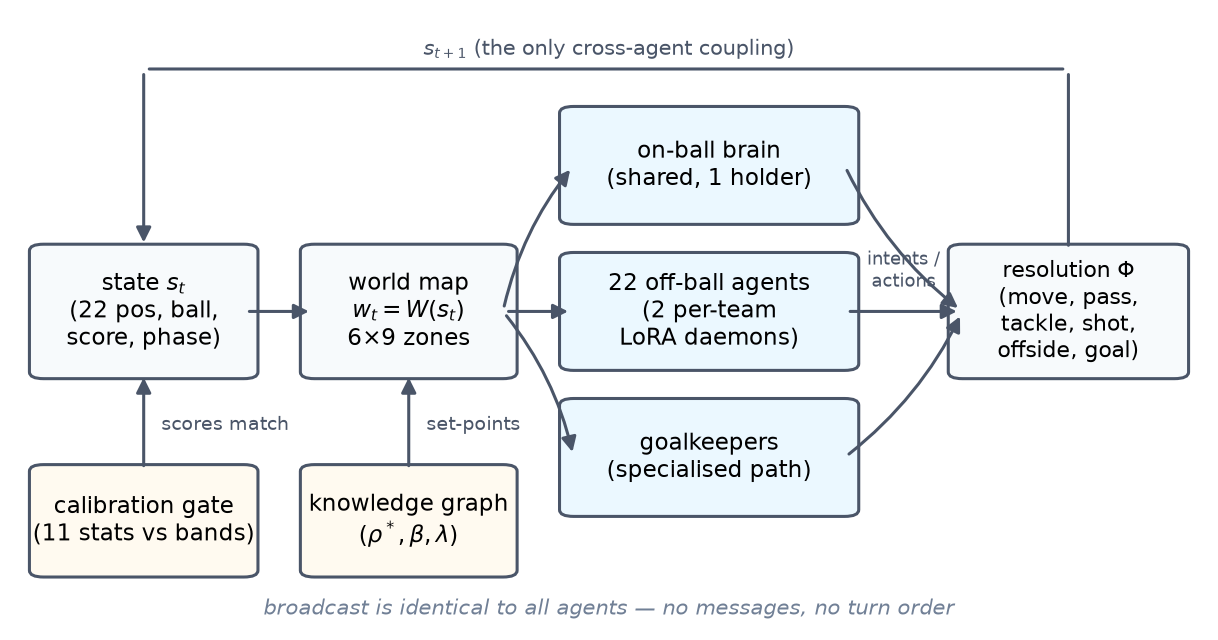
\includegraphics[width=0.96\textwidth]{fig_architecture.png}
\caption{\sfas{} 的智能体循环。一份共享世界地图被广播给二十二个彼此隔离的智能体（一个共享的持球“大脑”策略，与两个按队的无球策略，各为叠加在共享基座上的一个 LoRA）；它们的意图仅由确定性解算算子 $\Phi$ 合并，后者推进状态。知识图谱提供战术设定点；校准门为已完成的比赛打分。经由 $\Phi$ 的递归是\emph{唯一}的跨智能体耦合。}
\label{fig:arch}
\end{figure}

\paragraph{为何朴素搭建会失败。} 直接拼装时，该循环以两种典型方式失败，且二者都是\emph{动力学}问题、而非实现问题。其一，控球\emph{滚雪球}：早早赢得球权的一方会保有球权直到终场（最终份额 $80$--$90\%$），因为持球是自我强化的——控球方维持其阵型与逼抢，因而更可能赢得下一次对抗。其二，若逐字执行智能体的空间意图，每名球员都会汇聚到球上——LLM 被问“你该去哪”，合情合理地回答“去球那里”——于是阵型坍缩成一点，毁掉了使足球成其为足球的空间结构。二者都不是待打补丁的 bug；每一个都是某一类动力系统的一般行为，且各由一条带有清晰闭式阈值的控制律治愈。辨识这些阈值、并把它们与系统实际使用的工程常数联系起来，正是本文的技术核心。

\paragraph{贡献。}
\begin{itemize}
\item \textbf{一个系统。} \sfas：一个多智能体 LLM 足球模拟器，其中协调由共享环境而非通信承载，球队身份是可热插拔的低秩适配器，战术锚定于知识图谱（\S\ref{sec:arch}--\ref{sec:kgsec}）。我们将其形式化为一个\emph{stigmergic 马尔可夫博弈}，并证明在共享地图条件下联合策略按智能体分解（命题~\ref{prop:factor}）；进一步说明知识图谱、按队 LoRA 与无消息框架如何组合成互补的宏观/微观/在线三层（\S\ref{sec:kgsec}）。该设计\emph{与 backbone 无关}——我们将大脑分别以 Nemotron-3 Super 与 Qwen3.5-35B-A3B 运行、球员以 Gemma-4-E2B 运行，任何满足决策接口的指令微调模型都可原样替入（\S\ref{sec:serve}）。
\item \textbf{为何稳定。} 我们证明涌现控球在强化强度 $\beta=1$ 处发生超临界 pitchfork 分岔——滚雪球是一般性的（定理~\ref{thm:bistable}）——并证明一条近期份额反馈律在其增益超过 $g^\star=4(\beta-1)$ 时恰好消除它（定理~\ref{thm:stabilise}），且一个主场优势标量即可设定目标（推论~\ref{cor:setpoint}）。我们证明意图锚定的不坍缩保证：对任意混合权重 $\lambda<1$，阵型离散度的下界为 $(1-\lambda)^2S^2$（命题~\ref{prop:noncollapse}）。这些把一串常数变成少数几条可辨识的控制律。
\item \textbf{验证。} 在覆盖七组世界杯对阵、共 $75$ 场的语料上，标准统计量落入真实区间；一次六场消融复现了所预言的控球垄断；战绩追随实力同时保有真实的爆冷率（五组一边倒对阵中 $11\%$），控球、射门与 xG 分布真实（\S\ref{sec:exp}）。该框架可推广至任意对阵；新对阵以增量方式纳入。
\end{itemize}

\section{相关工作}\label{sec:related}

\paragraph{LLM 智能体与智能体社会。} Generative agents 以 LLM 驱动的角色填充一座沙盒小镇，其行为从记忆与规划中涌现 \citep{park2023}；开放式具身智能体在 Minecraft 中行动 \citep{wang2023voyager}；综述则梳理了这一迅速扩张的领域 \citep{wang2023survey}。许多多智能体 LLM 系统通过\emph{通信}协调——角色扮演对话、辩论或消息传递 \citep{li2023camel}——而单个智能体则经由如 ReAct \citep{yao2023} 的工具使用循环来推理与行动，这也是我们赛后分析智能体所采用的方式。\sfas{} 的不同之处在于其二十二个智能体从不通信；协调完全由共享环境中介。

\paragraph{多智能体学习与团队博弈。} 涌现集体行为已由强化学习在《星际争霸 II》\citep{vinyals2019}、《Dota 2》\citep{berner2019} 与捉迷藏 \citep{baker2020} 中大规模展示，而足球自 RoboCup \citep{kitano1997} 起、近来又有 Google Research Football 环境 \citep{kurach2020}，一直是一个测试平台。这些系统从奖励中\emph{优化}底层策略；我们则\emph{规定} LLM 智能体并\emph{分析}涌现不变量，以样本昂贵的训练换取可解释性与直接的战术控制。

\paragraph{去中心化控制、stigmergy、平均场。} 在无通信下控制一个共享马尔可夫过程即 Dec-POMDP 模型，其最坏情形为 NEXP 完全 \citep{bernstein2002}；\sfas{} 是其一个可处理的 \emph{stigmergic} 子类，其中一份精心设计的共有观测取代了通信，与群体生物学中的 stigmergy 一脉相承 \citep{theraulaz1999}。将二十二个相互作用的智能体约化为一个标量平均场，沿用了平均场博弈与平均场多智能体强化学习的思想 \citep{lasry2007,yang2018mfmarl}。

\paragraph{适配、知识图谱与足球统计。} 球队身份由叠加在量化共享基座 \citep{dettmers2023qlora} 之上的低秩适配 \citep{hu2021} 编码；战术先验从知识图谱检索，承袭检索增强生成 \citep{lewis2020} 与基于图的 RAG \citep{edge2024graphrag}。真实区间取自足球进球的经典统计规律 \citep{maher1982,dixon1997}，比分差服从 Skellam 分布 \citep{skellam1946}。我们的控球分析使用强化过程理论 \citep{pemantle2007} 与随机逼近的 ODE 方法 \citep{benaim1999,kushner2003}；其分岔即标准的 pitchfork \citep{strogatz1994}；标定 policy 的搜索用交叉熵法 \citep{rubinstein2004}。据我们所知，涌现控球的双稳态、其闭式稳定化阈值，以及意图锚定的不坍缩保证均为新结果。

\section{系统架构}\label{sec:arch}

\subsection{状态、共享世界地图与解算算子}

\sfas{} 是一个以离散\emph{帧}推进的\emph{实时}模拟，正如游戏引擎逐帧渲染一场比赛：一帧是对连续演化的比赛的一个瞬时采样，而非某名球员的“回合”。全部二十二个智能体在\emph{每一}帧上同时、独立地感知并行动——没有出手顺序、没有轮流、也没有任何智能体等待另一个。一帧把物理时间推进一个小的固定增量，一场完整九十分钟比赛跨越约 $4000$ 帧；这种离散性是一个固定的模拟时间步——正如游戏引擎逐帧推进其世界——而非回合结构。下文下标 $t$ 即按此意义为帧编号。

第 $t$ 帧的\emph{状态}为 $s_t=(\{x_i^t,r_i\}_{i=1}^{22},\,b_t,\,c_t,\,\text{ph}_t)$：球员位置 $x_i^t\in P$ 落在球场 $P=[0,L_x]\times[0,L_y]$ 上，固定角色 $r_i$，球 $b_t=(\xi_t,\hat\imath_t)$（位置与持球者下标，散球时 $\hat\imath_t=\varnothing$），比分 $c_t$，赛段 $\text{ph}_t$。球员分为主队 $H=\{1,\dots,11\}$ 与客队 $A=\{12,\dots,22\}$，其中 $1,12$ 为门将。

智能体从不看到 $s_t$。它们看到一份\emph{共享世界地图} $w_t=\Wmap(s_t)$（图~\ref{fig:arch}）：一种确定性粗化，将每个连续位置替换为其在固定 $6\times9$ 区域网格中的格子，附上每名球员的角色与一个持球标志，并附上球的区域、比分与赛段。同一份 $w_t$ 原样广播给所有智能体。粗化是刻意的：它使每个智能体的输入低维且离散——这是可靠解码与 \S\ref{sec:lora} 中低秩风格适配器的前提——并且，如 \S\ref{sec:why} 所示，它是协调的唯一渠道。

状态由唯一的确定性\emph{解算算子} $\Phi:\Sphere\times\Aspace^{22}\to\Sphere$ 推进：它把每名球员朝其意图与阵型锚点的混合（\S\ref{sec:why}）方向移动一个有界步长，以技能加权的竞争解算至多一个持球动作，强制球至多有一个持有者的守恒律，并裁决抢断、传球、射门、越位与进球。我们记 $s_{t+1}=\Phi(s_t,\mathbf a_t)$。$\Phi$ 承载环境自身的随机性（技能竞争），也是二十二个动作\emph{唯一}相互作用之处；智能体的策略本身亦是随机的，但每个智能体的\emph{决策}仅经由 $w_t$ 依赖于他人。

\subsection{三种策略及其部署}\label{sec:serve}

\sfas{} 在同一份世界地图上运行三类策略。(a) 一个共享的\emph{持球}“大脑”策略决定唯一持球者的动作；它是一个以低延迟运行的较大模型，作为延迟优化仅每隔几帧重新查询一次——相对于移动，持球者的决策变化较慢，故其最近一次动作在中间各帧持续，而持球者仍在每一帧行动。这是算力节流，而非轮流出手。(b) 两个\emph{无球}策略，每队一个，决定其余每名球员的意图（目标区域加姿态）；它们即 \S\ref{sec:lora} 的球队适配器，作为两个独立守护进程（主、客）部署。(c) 门将走一条永不返回场上动作的专用路径。三者在本地独立部署；由于智能体不通信（命题~\ref{prop:factor}），一帧内全部二十二次查询并行发出，两个球队守护进程并发运行。这种分工——一个共享的重型策略服务于罕见的持球决策，两个廉价的专用策略服务于大量无球决策——正是使一场完整九十分钟、约 $4000$ 帧的比赛能在本地硬件上可行的关键。

\paragraph{模型无关的 backbone。} 三类策略经由一个狭窄统一接口触达其模型——结构化世界地图提示进、受 schema 约束的决策出——故架构不依赖任何特定模型族、厂商或检查点。在我们的运行中，持球大脑在两台独立机器上分别以 \emph{Nemotron-3 Super}（$120$B）与 \emph{Qwen3.5-35B-A3B} 部署，无球球队策略以 \emph{Gemma-4-E2B} 适配器部署；\S\ref{sec:why} 的涌现性质——稳定且落入区间的控球、完整的阵型、真实的聚合统计——在任一大脑下都定性不变，正如理论所预言，因为它们是控制律与共享环境的性质，而非 backbone 的性质。因此任何能发出该决策 schema 的指令微调模型都是即插即用的替代：满足同一接口的可比开源 backbone 在大脑层包括 \emph{Llama-4-Maverick}、\emph{Qwen3.5-72B}、\emph{Mistral-Large-2}、\emph{DeepSeek-V3.2} 与 \emph{MiniMax-M1}，在轻量（$3$--$10$B）球员层包括 \emph{Gemma-4-E4B}、\emph{Qwen3.5-9B}、\emph{GLM-4-9B}（智谱）、\emph{InternLM3-8B}、\emph{MiMo-7B}（小米）与 \emph{Hunyuan-7B}（腾讯）。由于身份存于秩 $16$ 适配器、战术存于知识图谱而非基座权重，更换 backbone 既不改球队库也不改控制律——只改适配器所扰动的那份共有能力。

\section{用按队 LoRA 编码球队身份}\label{sec:lora}

\sfas{} 的一个核心设计抉择是：\textbf{球队身份是一个参数，而非一段提示词}（图~\ref{fig:lora}）。我们不是用文字描述“像巴西那样踢”再寄望于基座模型照办，而是\emph{训练}一个小适配器，把基座策略的决策分布朝一支球队的特征性选择移动。

\begin{figure}[t]\centering
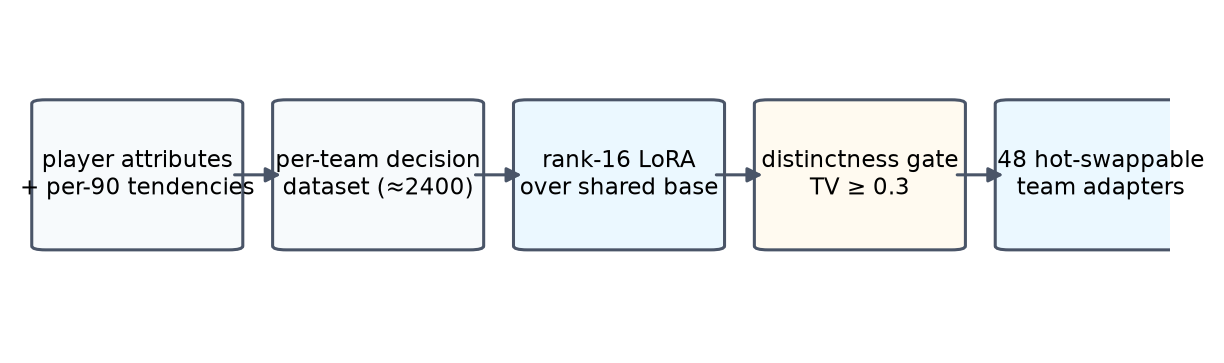
\includegraphics[width=0.96\textwidth]{fig_lora_pipeline.png}
\caption{按队身份流水线。球员属性与每 90 分钟统计倾向被蒸馏成一个按队的决策数据集（约 $2400$ 条），用于在同一共享基座上训练一个秩 $16$ 的 LoRA；所得按队策略须通过一道行为可区分性门方可被采纳。四十八支国家队各自成为一个可热插拔的适配器。}
\label{fig:lora}
\end{figure}

\paragraph{从属性到决策数据集。} 对每支球队，我们合成一个监督数据集（约 $2400$ 条）的（世界地图情境，决策）对。决策由一支球队球员的属性——射术、传球、抢断、速度与角色——以及每 90 分钟统计倾向（球队射门、突破、逼抢的频度）生成，从而，例如，进攻三区中一名高射术前锋被教导更果断地射门，一支高逼抢球队被教导更早地投入抢断。每条样本是一段简短的结构化提示（粗化情境）与系统动作词表中的一个目标决策。

\paragraph{在共享基座上的低秩适配。} 每支球队 $\tau$ 是一个低秩适配器 \citep{hu2021}：基座权重 $W_0$ 变为 $W_0+B_\tau A_\tau$，其中 $A_\tau\in\mathbb R^{r\times d}$、$B_\tau\in\mathbb R^{d\times r}$、秩 $r=16\ll d$，在冻结基座的同时用该队数据集监督微调而得。两条性质使其成为合适工具。其一，\emph{成本}：一个秩 $16$ 适配器只有几十兆字节，故全部四十八支国家队可与同一共享基座并存、在部署时热插拔——选定一场对阵是加载两个适配器，而非两个模型。其二，\emph{简约}：身份是对共享足球先验的一个\emph{扰动}，而非一个独立模型，这既起到正则化作用（基座提供共有能力），又使“风格”成为我们可推理的低维对象（\S\ref{sec:ident}）。

\paragraph{一道可区分性门。} 一个球队适配器只有在行为上\emph{可区分}时才被采纳部署：在一组固定的情境探针上，其决策分布须与其他每支球队相差至少一个间隔（总变差可区分度 $0.3$）。这道门（\S\ref{sec:ident} 分析）保证四十八个适配器张成真正不同的打法风格，而非塌回共享基座。

\section{知识图谱战术锚定}\label{sec:kgsec}

按队 LoRA 编码了球员\emph{是谁}；它本身并不编码\emph{球队作为一个整体打算如何踢}，也不让设计者陈述并编辑战术。\sfas{} 用一张\emph{战术知识图谱}提供这一层，而且——如下文所论——知识图谱并非装饰性附件，而是使按队 LoRA 与无消息智能体框架\emph{协同}发挥得比各自单独更好的那个组件（图~\ref{fig:kg}）。

\begin{figure}[t]\centering
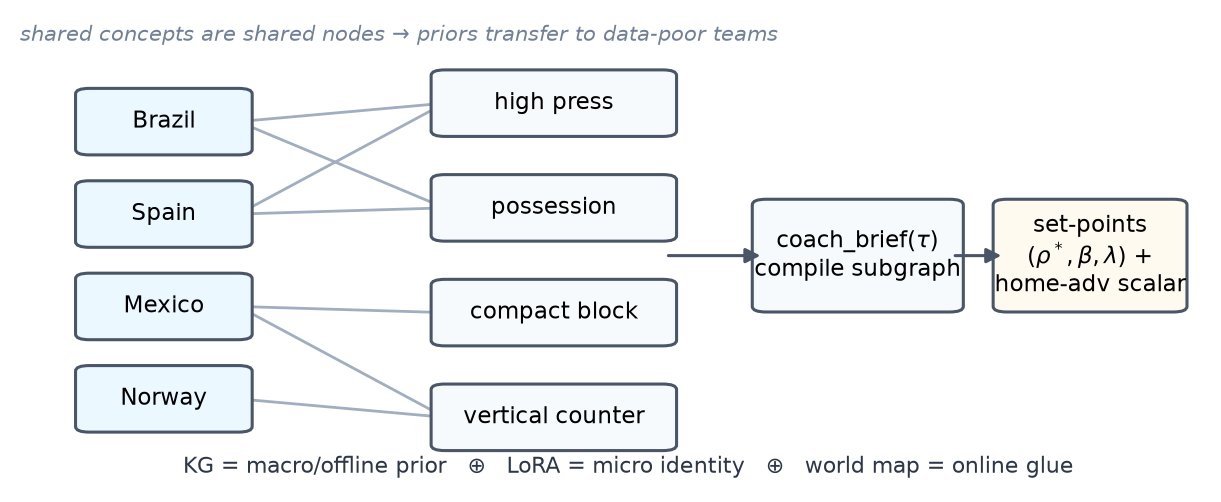
\includegraphics[width=0.98\textwidth]{fig_kg.png}
\caption{知识图谱及其协同。\textbf{(1)} 一张关系图把四十八支球队连到共享的战术\emph{概念}（高逼抢、控球、紧凑防守、纵向反击）；共享同一风格的球队共享一个节点，故战术知识得以\emph{迁移}，数据稀缺的球队经由其邻居继承先验。一次按队查询 \texttt{coach\_brief}$(\tau)$ 把相关子图编译成控制设定点 $(\hat\rho,\beta,\lambda)$ 与一个主场优势标量。\textbf{(2)} 这些设定点恰是 \S\ref{sec:why} 控制律所执行的、按队 LoRA 微观决策在其中运作的、以及对齐本来无消息智能体的对象。三层互补：宏观/离线先验 $\oplus$ 微观身份 $\oplus$ 在线黏合。}
\label{fig:kg}
\end{figure}

\subsection{图谱是什么、如何运作}

该图谱是覆盖全部四十八支球队的关系战术本体：节点为球队、战术\emph{概念}（如高位逼抢、控球保持、纵向反击、紧凑中场防守）、关键球员角色与特征性组合；边把一支球队连到它所体现的概念，并把共同出现的概念相连。关键在于，被若干球队共享的战术概念是\emph{一个}节点、带多条入边连向相关球队，故图谱是高度互联的，而非四十八份互不相干的画像。一道轻量、确定性的编译把每支球队的属性与风格描述符转成该图；一道可选的语言模型增强用叙事性战术文本充实它，随后建立索引以供混合（稠密 $+$ 稀疏）检索，沿用检索增强与基于图的 RAG 系统的方式 \citep{lewis2020,edge2024graphrag}。

比赛时一次读取 $\texttt{coach\_brief}(\tau)$ 检索球队 $\tau$ 周围的子图——其概念、其突出组合，以及经由共享概念边它所处的战术邻域——并把它编译成系统其余部分所消费的少数几个\emph{控制设定点}：一个控球目标（进入 \S\ref{sec:why} 的\emph{对阵}锚点，由学习所得标定 policy 从\emph{双方}风格向量编译）、一个逼抢水平（设定强化/换手机制 $\beta$）、以及一个阵型紧凑度（告知锚定权重 $\lambda$）。该读取是离线且自包含的——比赛循环内无需实时数据库——故图谱在不增加运行时耦合的情况下添加了战术锚定。

\subsection{它如何提升系统}

把战术锚定在图谱而非自由文本提示中，带来四样东西。\emph{(i) 一致性：} 每场比赛注入同样的战术事实，故球队的宏观行为是可复现的，而非每次都从提示中重新采样。\emph{(ii) 迁移：} 因为共享风格是共享节点，一支训练数据稀少的球队从其有更充分佐证的邻居处继承战术先验——图谱以一种按队工件无法做到的方式跨球队泛化。\emph{(iii) 可解释、可编辑的接口：} 设计者陈述“这一方高位逼抢并保有球权”，编辑一个节点，改动便确定性地传播进控制设定点——战术是可检视、可版本管理的，而非埋在权重里。\emph{(iv) 关注点分离：} 图谱承载\emph{球队级意图}，LoRA 承载\emph{球员级倾向}，故二者可独立开发、验证与替换。

\subsection{与 LoRA 和智能体框架的协同}

三个组件在不同层级运作并相互增强（图~\ref{fig:kg} 右）；这正是该组合为何奏效的核心。

\paragraph{图谱 $\oplus$ LoRA：宏观意图遇上微观身份。} LoRA 移动一名球员的\emph{微观}决策分布（高射术前锋更早射门）；图谱设定球队所处的\emph{宏观}范围（高位逼抢、目标控球 $59\%$）。二者互不包含：一个控球风格的设定点配上一名“直接打法”前锋的适配器，会产出仍以早射门收尾的耐心组织——这是任何单一提示都难以可靠诱出的组合。图谱还\emph{弥补 LoRA 的数据局限}：当某小型协会的适配器较薄弱时，共享概念边迁移来一个合理的战术先验，故即便其微观策略训练不足，球队仍然连贯。具体而言，图谱选定目标 $\hat\rho$ 与 $\beta,\lambda$ 设定点；LoRA 在其条件下选定每帧动作\emph{分布}；校准门（\S\ref{sec:calib}）检查联合结果。

\paragraph{图谱 $\oplus$ 智能体框架：球队级的相关化装置。} 智能体是无消息的（命题~\ref{prop:factor}）：一帧内它们仅经由共享世界地图协调，而后者承载\emph{位置}而非\emph{策略}上的共有知识。因此不存在一条赛中通道，让十一名队友约定，比方说，作为一个整体高位逼抢。知识图谱恰好填补这一空缺：它是一个\emph{离线、球队级的相关化装置}，一份赛前的教练指令，经由共享设定点被全队每个智能体内化，而世界地图则是\emph{在线、逐帧级}的相关化装置。两个相关化装置作用于不同时间尺度、互为补充——没有图谱，智能体在位置上协调而在战术上不协调；没有共享地图，它们无法逐帧执行战术。用 \S\ref{sec:why} 的语言：图谱设定\emph{设定点}，世界地图承载\emph{状态}，LoRA 提供\emph{策略}，而 \S\ref{sec:why} 的控制律保证涌现结果稳定。这一分工——宏观/离线先验 $\oplus$ 微观身份 $\oplus$ 在线黏合，并由一个外层校准回路保持诚实——正是 \sfas{} 的核心架构思想。

\section{系统为何稳定}\label{sec:why}

本节解释 \S\ref{sec:intro} 的两个失败模式以及治愈它们的控制律。我们把陈述留在正文、把完整证明推迟到附录~\ref{app:proofs}；这里强调机制与图。

\subsection{无通信的协调}\label{sec:stig}

一个 \emph{stigmergic 马尔可夫博弈}是这样一个马尔可夫博弈：每个智能体观测同一份地图 $w_t=\Wmap(s_t)$，没有其他输入（无通信，一帧内不窥探他人的动作或记忆），且状态由固定算子 $s_{t+1}=\Phi(s_t,\mathbf a_t)$ 推进。

\begin{proposition}[策略分解]\label{prop:factor}
在一个 stigmergic 马尔可夫博弈中，联合动作分布在世界地图条件下按智能体分解，$\Prob(\mathbf a_t\mid s_t)=\prod_{i=1}^{22}\pi_i(a_i\mid\Wmap(s_t))$，因而一步转移为 $\Prob(s_{t+1}\mid s_t)=\sum_{\mathbf a}\mathbf1\{s_{t+1}=\Phi(s_t,\mathbf a)\}\prod_i\pi_i(a_i\mid\Wmap(s_t))$。已实现轨迹中的全部跨智能体依赖由 $\Phi$ 与递归产生；决策步内不产生任何依赖。共享地图充当一个相关化装置。
\end{proposition}

这是 \S\ref{sec:serve} 中并行、无消息部署的形式化许可，并告诉我们协调失败位于何处：不在任何单个 $\pi_i$ 中，而在乘积策略与 $\Phi$ 随时间的相互作用里。下面两个病态恰是这样的相互作用效应。

\subsection{控球是双稳态的——而一条反馈律能修复它}\label{sec:poss}

设 $\b_t\in\{0,1\}$ 表示第 $t$ 帧主队是否持球（散球帧不计入）。系统以权重 $\alpha$ 的指数加权估计量追踪主队的\emph{近期控球份额}，
\begin{equation}\label{eq:ema}
\rho_{t+1}=(1-\alpha)\rho_t+\alpha\,b_{t+1},\qquad\rho_0=\tfrac12 .
\end{equation}
由于占优一方维持其阵型与逼抢，它赢得下一次对抗的概率随其近期份额上升；我们以换手 hazard $h_H(\rho)=h_0e^{-\beta(2\rho-1)}$、$h_A(\rho)=h_0e^{+\beta(2\rho-1)}$ 刻画之，故下一持球者概率为 $q(\rho)=h_A/(h_A+h_H)=\sigma(4\beta(\rho-\tfrac12))$，其中 $\sigma$ 为 logistic 函数、$\beta\ge0$ 为\emph{强化强度}。按帧编号的过程~\eqref{eq:ema} 的渐近行为由一个一维平均场支配。

\begin{lemma}[平均场约化]\label{lem:meanfield}
近期份额过程~\eqref{eq:ema} 是一个常增益 Robbins--Monro 递归，其平均场为梯度流
\begin{equation}\label{eq:meanode}
\dot\rho=m(\rho):=q(\rho)-\rho=\sigma\!\big(4\beta(\rho-\tfrac12)\big)-\rho .
\end{equation}
$\{\rho_t\}$ 的插值轨迹几乎必然收敛到 $m$ 的不动点集，且不会收敛到线性不稳定者；在稳定不动点 $\rho^\ast$ 附近其稳态涨落方差为 $\alpha\,q(\rho^\ast)(1-q(\rho^\ast))/(2|m'(\rho^\ast)|)+O(\alpha^2)$，即 $O(\sqrt\alpha)$ 带。
\end{lemma}

\noindent（证明见附录~\ref{app:proofs}，用随机逼近的 ODE 方法 \citep{benaim1999,kushner2003}。）因此 $m$ 各均衡的稳定性决定涌现控球；下面分析之。

\begin{theorem}[涌现控球的双稳态]\label{thm:bistable}
均衡态 $\rho=\tfrac12$ 是 $\dot\rho=m(\rho)$ 的不动点，当且仅当 $\beta<1$ 时线性稳定。当 $\beta$ 越过 $1$，系统发生超临界 pitchfork：$\beta>1$ 时均衡态不稳定，并出现两个稳定不动点 $\rho_\pm(\beta)$，当 $\beta\to\infty$ 时 $\rho_\pm\to\{0,1\}$。因此对任意 $\beta>1$，未受控的模拟器几乎必然把控球驱向近乎垄断（图~\ref{fig:bif}）。
\end{theorem}

定理~\ref{thm:bistable}（图~\ref{fig:bif}）是滚雪球的精确陈述：只要持球哪怕轻微自我强化，一个\emph{未受控}的模拟器\emph{必定}把控球驱向垄断，胜者由早期噪声决定。任何提示工程都无法消除它；它是平均场的性质，必须在动力学层面治愈。

\begin{figure}[t]\centering
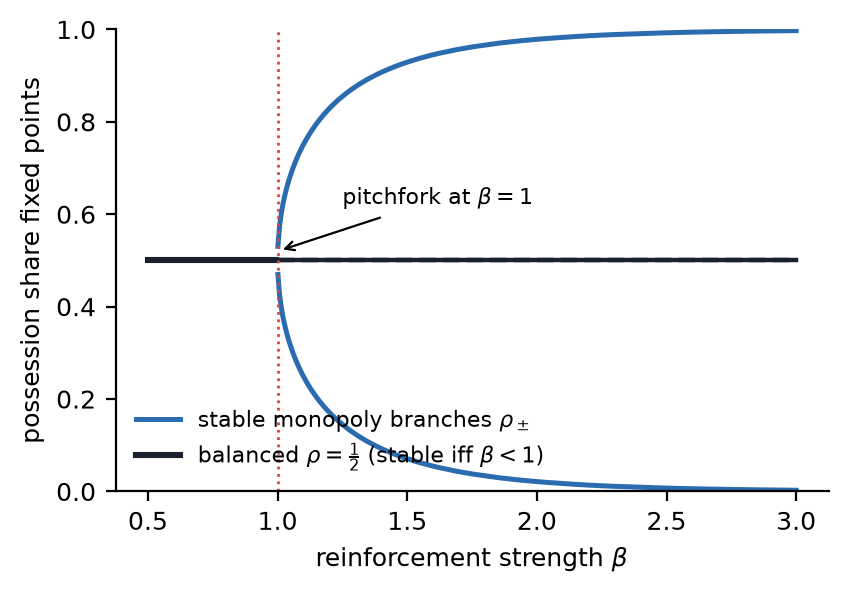
\includegraphics[width=0.72\textwidth]{fig_bifurcation.png}
\caption{开环控球平均场在强化强度 $\beta=1$ 处发生超临界 pitchfork：$50\%$ 的均衡（$\beta<1$ 时稳定）失稳，并涌现两条稳定的控球垄断分支——即滚雪球失败模式（定理~\ref{thm:bistable}）。}
\label{fig:bif}
\end{figure}

治愈之道是一条\emph{对抗}占优的反馈：一旦某队近期份额越过死区 $\rho^\star$，就按超出量成比例地抬高\emph{它}的换手 hazard，$h_H(\rho)\mapsto h_H(\rho)(1+g(\rho-\rho^\star)_+)$，客队对称，其中 $g\ge0$ 为\emph{反馈增益}。

\begin{theorem}[稳定化与临界增益]\label{thm:stabilise}
设 $\beta>1$、$\rho^\star=\tfrac12$。在该反馈下，均衡态是受控平均场的不动点，且线性稳定当且仅当
\begin{equation}\label{eq:gstar}
g>g^\star=4(\beta-1).
\end{equation}
当 $g>g^\star$ 时，它是\emph{唯一}的稳定均衡，垄断态 $\rho_\pm$ 被摧毁，闭环控球~\eqref{eq:ema} 集中在目标的 $O(\sqrt\alpha)$ 邻域内。
\end{theorem}

式~\eqref{eq:gstar} 是核心的实用陈述：把对抗占优的增益取得大于强化超额 $\beta-1$ 的四倍，一个注定的垄断便成为一场受控的真实比赛。系统采用 $g=22$、$\alpha=0.02$（约 $50$ 帧窗口）、$\rho^\star=0.55$；$g=22$ 对每个直到 $\beta=6.5$ 的强化强度都越过 $g^\star$——远超现实区间——而小 $\alpha$ 给出我们观测到的 $O(\sqrt\alpha)\approx0.14$ 单场波动带。图~\ref{fig:feedback} 通过对~\eqref{eq:ema} 的 Monte-Carlo 直接确认了分岔及其消除：当 $g=0<g^\star$ 时最终控球直方图在垄断处双峰；当 $g=22>g^\star$ 时则在设定点处单峰。

\begin{figure}[t]\centering
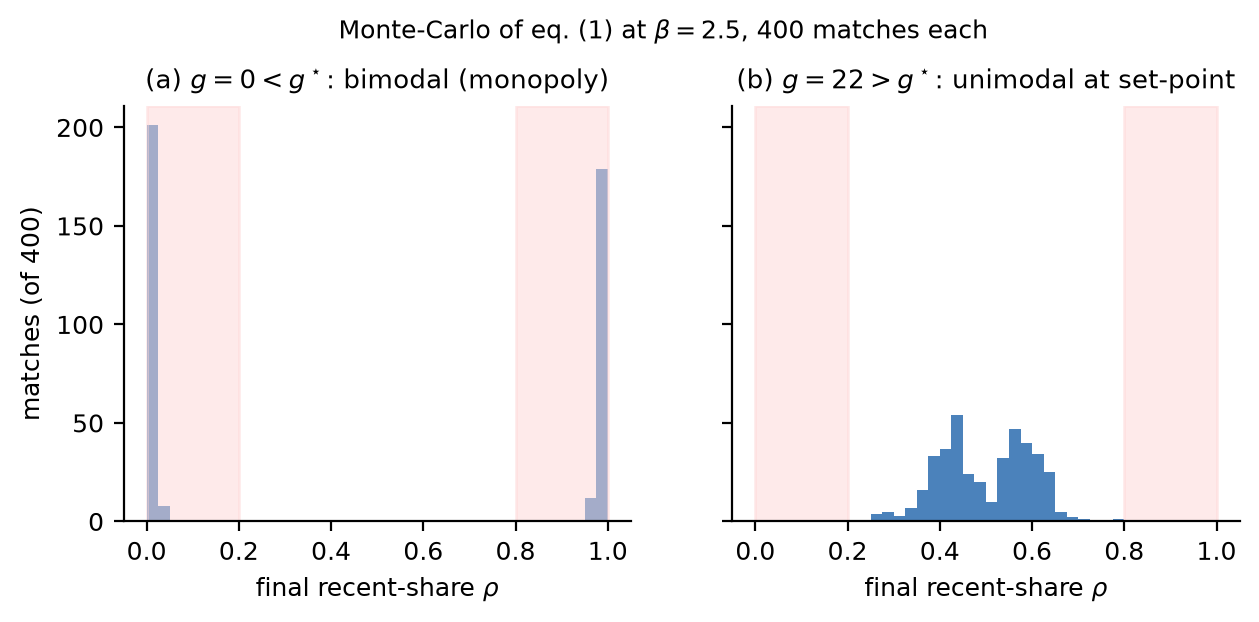
\includegraphics[width=0.92\textwidth]{fig_feedback.png}
\caption{在 $\beta=2.5$ 下对控球过程~\eqref{eq:ema} 的 Monte-Carlo（各 $400$ 场）。(a) 无反馈（$g=0<g^\star$）时最终控球呈双峰——早早领先的一方垄断球权。(b) 有反馈（$g=22>g^\star$）时呈单峰并集中于设定点，恰如定理~\ref{thm:stabilise} 所预言。}
\label{fig:feedback}
\end{figure}

\begin{corollary}[主场优势设定点]\label{cor:setpoint}
一个小的主场优势 $h_H\mapsto h_H(1-\eta_H)$、$h_A\mapsto h_A(1+\eta_A)$ 把唯一稳定不动点移至 $\rho^\dagger=\tfrac12+(\eta_H+\eta_A)/(2(g-g^\star))+O(\eta^2)$。因此一个主场优势标量即可连续且单调地移动校准后的控球目标。
\end{corollary}

推论~\ref{cor:setpoint} 是从知识图谱到物理的桥梁：一条战术指令（“控制球权”）映射为一个期望份额，再经上述单调关系映射为一个标量，而定理~\ref{thm:stabilise} 随后把它稳稳保持住。\emph{图谱设定点，控制律执行之。}

\paragraph{对阵相关标定——由学习给出，而非手工设定。} 推论中的设定点不是全局常数：它按\emph{对阵}、由双方的真实风格向量（$48$ 队实测控球/传球成功率/实力统计库）编译而得。编译目标为
\[
\hat\rho(h,a)=\operatorname{clip}\!\big(\tfrac12+\kappa\,[\,w_p\Delta_{\text{控球}}+w_c\Delta_{\text{传球}}+w_z\Delta_z\,]+\eta_{\text{主场}},\ \tfrac12\pm b\big),\qquad b=0.065,
\]
经推论~\ref{cor:setpoint} 的机制实现为闭环不动点 $\rho^\dagger$——西班牙--奥地利与巴西--日本得到\emph{不同}的标定，而任意两组对阵的目标差被限制在 $13$ 个百分点内。执行刻意柔和——\emph{被引导的涌现}：目标只设一个低增益导演（$k_p=0.4$，教练式轻推而非强拉）与一条弱化的物理倾斜；三条风格通道则作为\emph{行为}修饰注入——逼抢以 $(1+0.6\,(\mathrm{press}-\tfrac12))$ 缩放对手的丢球 hazard、并以 $(1-0.30\,(\mathrm{press}-\tfrac12))$ 收紧盯人距离进入上下文传球完成率模型；节奏缩放持球方出球 hazard；直接度重排传球目标评分——控球差由此\emph{从行为博弈中涌现}，而非被强加。分工在数字上一目了然：最悬殊的对阵里，编译目标在 clip 处饱和（$56.5\%$），而涌现落位是 $68.2$--$68.6\%$（\S\ref{sec:exp}）——目标最多贡献落位的 $6.5$ 个百分点，其余约 $12$ 个百分点由三条行为通道经对抗产生。八个标定参数 $\theta=(\kappa,w_p,w_c,w_z,\text{倾斜尺度},\text{三个风格增益})$ 由交叉熵法策略搜索 \citep{rubinstein2004} 在引擎 rollout 上\emph{学习}而得：逐对阵损失 $=|\text{涌现份额}-\text{真实世界锚点}|$ 加垄断惩罚与传球成功率出带惩罚。训练用三组实力跨度不同的对阵——\emph{西班牙--奥地利}、\emph{巴西--日本}与语料之外的\emph{卡塔尔--西班牙}——因此\emph{七组评估对阵中有五组是 held-out}，包括场地对称性检验所依赖的两组重悬殊对阵（\emph{阿根廷--佛得角}、\emph{巴拉圭--法国}）；损失四轮内 $0.232\to0.150$（种群 $8$），学得 $\kappa=1.18$、$w_p=0.44$、$w_c=0.11$、$w_z=0.01$、逼抢/直接度/节奏增益 $0.69/0.38/0.50$（policy 存档于 \texttt{calib\_policy.json}，训练器 \texttt{calibrate\_policy.py}）。学出的目标依赖风格差而几乎不用原始实力差（$w_z\approx0$）是符合预期的——控球与传球风格本就编码了实力——因此 \S\ref{sec:exp} 的实力差伸缩经由风格通道传导，而非单独的实力项。\S\ref{sec:exp} 的两条可观察结论——优势方落位随实力差平滑变化、及其主客对称（主场 $68.2\%$ 对客场 $68.6\%$，且都在 held-out 对阵上）——来自这一对阵相关、学习所得的整套 policy：目标\emph{加}行为增益，而非目标单独。

\begin{remark}[死区、工作点与 $\beta$ 的实测]\label{rem:deadband}
定理~\ref{thm:stabilise} 分析对称死区 $\rho^\star=\tfrac12$，此时阈值恰为 $g^\star=4(\beta-1)$。部署系统用 $\rho^\star=0.55$：在 $[1-\rho^\star,\rho^\star]$ 内反馈不激活，故均衡态\emph{局部}不稳定（开环斜率 $m'(\tfrac12)=\beta-1>0$），份额向外漂移，直到在死区边缘反馈介入并将其制止。因此稳定工作点恰位于死区之外、靠近 $\rho^\star$——这正是为何在部署中，各组对阵的落位贴着各自的编译目标——巴西--日本（目标 $55\%$）落位边缘外侧 $59\%$、科特迪瓦--挪威（$53\%$）落位 $52\%$、墨西哥--厄瓜多尔（$50\%$）落位 $54\%$（推论~\ref{cor:setpoint}）。我们由六场开环（$g=0$）消融比赛\emph{实测}强化强度（$4{,}325$ 持球拍；$W=100$ 下 $36$ 个窗口转移对）。超临界的主证据是行为性的（图~\ref{fig:betaabl}）：六场中五场漂向极端——$69\%$ 的份额窗口落在 $\rho\le0.35$ 或 $\rho\ge0.65$、仅 $5\%$ 保持中央，领先模态份额 $\rho^+=0.68$——对比闭环在均势对阵上的单峰（极端 $11\%$、中央 $33\%$）；按定理~\ref{thm:bistable} 的反向读法，此类漂移仅在 $\beta>1$ 时发生。点估计符号一致：份额转移映射 $q(\rho)=\sigma(4\beta(\rho-\tfrac12))$ 在 $\rho^\star=\tfrac12$ 处的局部斜率（直接估计器）给出 $\hat\beta\approx1.6$--$2.3$，模态不动点关系 $\beta=\operatorname{logit}(\rho^+)/\big(4(\rho^+-\tfrac12)\big)$ 给出 $\hat\beta\approx1.05$；\emph{全局} logistic 拟合为 $0.77$--$0.91$——在此构造下必然低估，因为它把漂移被截断的饱和分支也并入拟合（与 AR(1) 斜率作为下界 $\approx0.7$--$0.8$ 同一机制）。一项合成恢复实验（同一估计管线跑由份额转移映射 $q(\rho)$ 按已知 $\beta$ 生成的轨迹；存档于 \texttt{beta\_estimator\_calibration.txt}）证实了这一判读：AR(1) 即使在真值 $\beta=2$ 时也只返回 $0.93$--$1.00$（$<1$）；在引擎式分支饱和下，模态估计器无论真值 $\beta\in[1.5,2]$ 都压缩到 $\approx1.05$——与我们实测的 $1.047$ 吻合——而亚临界对照（$\beta=0.8$）只产生 $29$--$38\%$ 极端窗口且局部斜率 $<1$，对比超临界的 $83$--$100\%$ 与 $\approx1.9$（实测：$69\%$ 与 $1.6$--$2.3$）。数据因此与真·超临界系统一致、与亚临界系统不一致。结论对这一散布不敏感：即便取最大估计，$g^\star=4(\hat\beta-1)\approx5.1$，而部署 $g=22$ 对任何 $\beta\le6.5$ 都超过 $g^\star$——反馈远在临界增益之上，这正是闭环控球稳落区间的原因。
\end{remark}

\begin{figure}[t]\centering
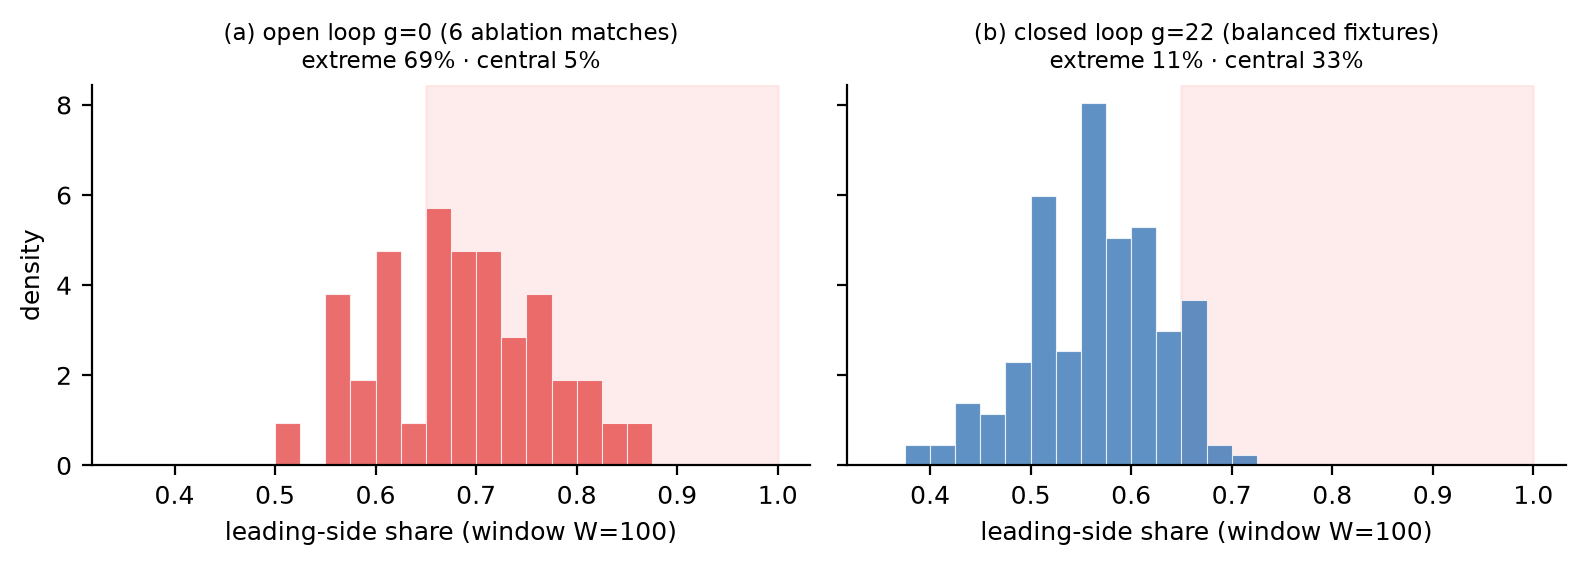
\includegraphics[width=0.94\textwidth]{fig_beta_ablation.png}
\caption{领先方份额分布（$W=100$ 持球帧窗口）。(a) 开环（$g=0$，六场消融）：质量漂向极端——$69\%$ 的窗口落在 $\rho\le0.35$ 或 $\rho\ge0.65$、仅 $5\%$ 中央——定理~\ref{thm:bistable} 对 $\beta>1$ 预言的双峰签名。(b) 闭环（$g=22$，两组均势对阵）：单峰，极端 $11\%$ / 中央 $33\%$；垄断区（阴影）保持为空。}
\label{fig:betaabl}
\end{figure}

\subsection{阵型不会坍缩}\label{sec:collapse}

无球时每个智能体发出目标 $z_i^t$；逐字执行“去球那里”会坍缩阵型。解算算子转而把每名球员朝其目标与固定阵型锚点 $\phi_i$ 的\emph{凸混合}方向移动，步长 $\eta$、混合权重 $\lambda$：
\begin{equation}\label{eq:anchor}
x_i^{t+1}=(1-\eta)x_i^t+\eta\big[(1-\lambda)\phi_i+\lambda z_i^t\big].
\end{equation}

\begin{proposition}[不坍缩保证]\label{prop:noncollapse}
设每个智能体都瞄准一个共同点（最坏情形，如全员追球），并带有跨球员方差为 $\sigma_z^2$ 的有界特异异质性。则~\eqref{eq:anchor} 的稳态阵型离散度为 $S_\infty^2=(1-\lambda)^2S^2+\lambda^2\sigma_z^2\ge(1-\lambda)^2S^2$，其中 $S^2$ 为阵型锚点的离散度。因此对任意 $\lambda<1$ 阵型不会坍缩；坍缩需 $\lambda=1$ 且 $\sigma_z=0$，是一个零测度情形。
\end{proposition}

命题~\ref{prop:noncollapse}（图~\ref{fig:disp}）把设计常数 $\lambda<1$ 变成一条保证，并量化了权衡：更大的 $\lambda$ 赋予智能体对阵型更多的话语权（更强的战术表达力），代价是更小的保证离散度 $(1-\lambda)^2$。\sfas{} 锚定两次（意图形成时一次 $\lambda_1=0.45$ 混合，运动模型中再一次 $\lambda_2=0.40$），故保留结构的因子相乘为 $((1-\lambda_1)(1-\lambda_2))^2\approx0.11$：即便全员追球，球队仍保有约 $11\%$ 的阵型展开，这既阻止了“二十二人全压球上”的退化态，又仍让战术得以形变阵型。

\begin{figure}[t]\centering
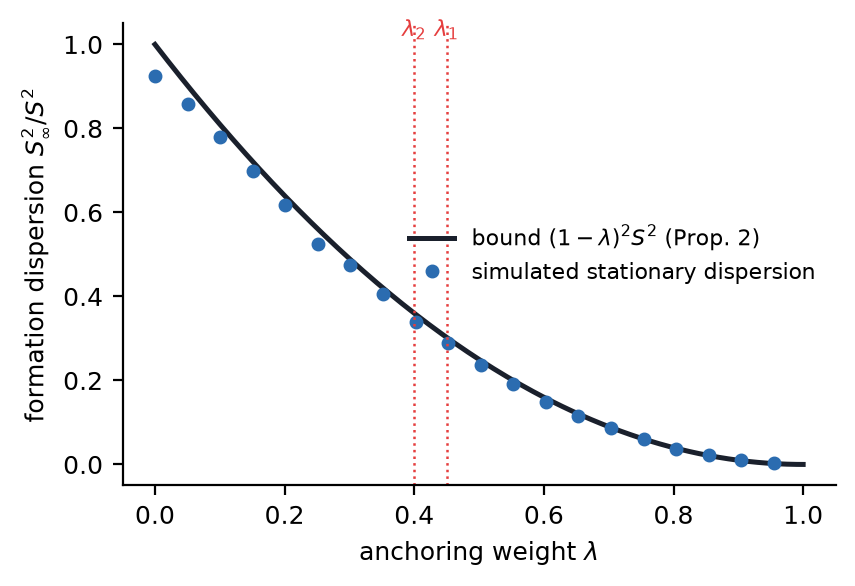
\includegraphics[width=0.66\textwidth]{fig_dispersion.png}
\caption{意图锚定对任意混合权重 $\lambda<1$ 保证阵型离散度有正下界 $(1-\lambda)^2S^2$（命题~\ref{prop:noncollapse}）；唯有在边界情形 $\lambda=1$ 才可能坍缩。\sfas{} 的两阶段锚定即便在全员追球时也保留约 $11\%$ 的阵型展开。}
\label{fig:disp}
\end{figure}

\subsection{校准作为外环}\label{sec:calib}

上述控制律被调校得使\emph{聚合}统计量落入独立设定的真实区间（表~\ref{tab:bands}）。两处耦合值得注意。控球区间\emph{与}控球段数都由定理~\ref{thm:stabilise} 支配——不动点设定平均份额，而该点处的换手 hazard 设定控球易手的频度。射门统计只因命题~\ref{prop:noncollapse} 使阵型不坍缩才有意义；一个坍缩的阵型会非物理地制造或抑制射门。因此校准并非十一项独立调参，而是少数几条可辨识控制律，其参数由区间锁定。

\begin{table}[h]\centering
\caption{校准门所执行的真实区间（除注明外为按队、按场），及其支配律。区间是\emph{典型}比赛的参考范围，与公开赛事数据（Opta/FBref）及 2022 世界杯一致；合理的极端值落在其外——控球占优的强队达 $\sim$70--80\%（如世界杯的西班牙），深度防守队低于 $30\%$，而对少数尝试求比的逐场比率（扑救率、射正率）有重尾（\S\ref{sec:exp}）。}
\label{tab:bands}
\small
\begin{tabular}{lcc}
\toprule
统计量 & 真实区间 & 支配律 \\
\midrule
控球率 & $30$--$70\%$ & 定理~\ref{thm:stabilise}、推论~\ref{cor:setpoint} \\
射门 & $5$--$20$ & 射门门 $+$ 离散度（命题~\ref{prop:noncollapse}） \\
射正率 & $25$--$50\%$ & 射术竞争 \\
扑救率 & $60$--$80\%$ & 门将竞争 \\
传球成功率 & $50$--$90\%$ & 上下文断球（逐脚实测） \\
越位频次 & $0$--$5$ & 防线几何 \\
控球段数 & $60$--$220$ & 定理~\ref{thm:stabilise}（换手率） \\
进球 & $0$--$7$ & 终结竞争（Skellam 差 \citep{skellam1946}） \\
期望进球（xG） & 与进球一致 & 射门质量模型 \\
回收球时间（秒） & $5$--$60$ & 换手 hazard \\
\bottomrule
\end{tabular}
\end{table}

\section{实验}\label{sec:exp}

\paragraph{设置。} 球队适配器以秩 $r=16$ 在同一共享基座上、由按队决策数据集（各约 $2400$ 条）为 2026 世界杯四十八支决赛圈球队蒸馏而得。逐对阵控球锚点由 \S\ref{sec:why} 的学习所得标定 policy 从双方真实风格向量编译（CEM 拟合，存档于 \texttt{calib\_policy.json}），并柔和执行（$k_p=0.4$ 导演、弱化倾斜、风格$\to$行为增益）。每场运行约 $4000$ 帧（九十分钟当量）；持球大脑是单一共享模型——此处以 \emph{Nemotron-3 Super} 运行，并在第二台机器上以 \emph{Qwen3.5-35B-A3B} 运行，行为一致——两个无球策略为 \emph{Gemma-4-E2B} 适配器、作为独立守护进程部署（\S\ref{sec:serve}）；backbone 可互换。每场比赛连同其完整逐帧轨迹、十一项统计行、运行配置与动态回放一并归档；下列全部图表可由语料复现。语料为覆盖实力谱系的七组对阵共 $75$ 场：\emph{巴西}--\emph{日本}、\emph{科特迪瓦}--\emph{挪威}、\emph{墨西哥}--\emph{厄瓜多尔}、\emph{西班牙}--\emph{奥地利}、\emph{比利时}--\emph{塞内加尔}与\emph{阿根廷}--\emph{佛得角}（各十场），外加十五场\emph{巴拉圭}--\emph{法国}系列。由于每场比赛都以同一模式归档，扩充语料纯属增量，不改动系统任何部分。

\paragraph{统计真实性（图~\ref{fig:bands}）。} 全部 $75$ 场中，聚合统计量落入其真实区间。传球成功率在全部 $150$ 个队·场均在带内（$64.6$--$87.4\%$，均值 $76.3\%$）；优势方控球随实力差伸缩（均势至中间梯队的逐对阵均值 $52$--$60\%$，最悬殊对碰达 $68$--$69\%$），且每场都留在 $30$--$70\%$ 内；控球段数、越位与回收球贴合各自区间；进球与 xG 一致（$149$ 球对 $207$ xG，每队·场 goals$-$xG 为 $-0.39$——终结带噪且略保守）。两处可理解的逐场例外仍在。第一处是射门数，在最高节奏的比赛中超出保守的 $5$--$20$ 区间——这忠实于真实足球，开放比赛会产生 $25+$ 次射门——在悬殊对阵中防守大巴一侧则低于它。第二处是扑救率：作为一场比赛内对少数射正次数之比，它本就高方差，并在少射门比赛中达到 $100\%$（小分母效应，恰如真实的零封）。二者都是小计数下逐场比率的性质，而非动力学的性质；表~\ref{tab:bands} 中赛季式区间描述的是\emph{典型}值，而均值遵从之。

\begin{figure}[t]\centering
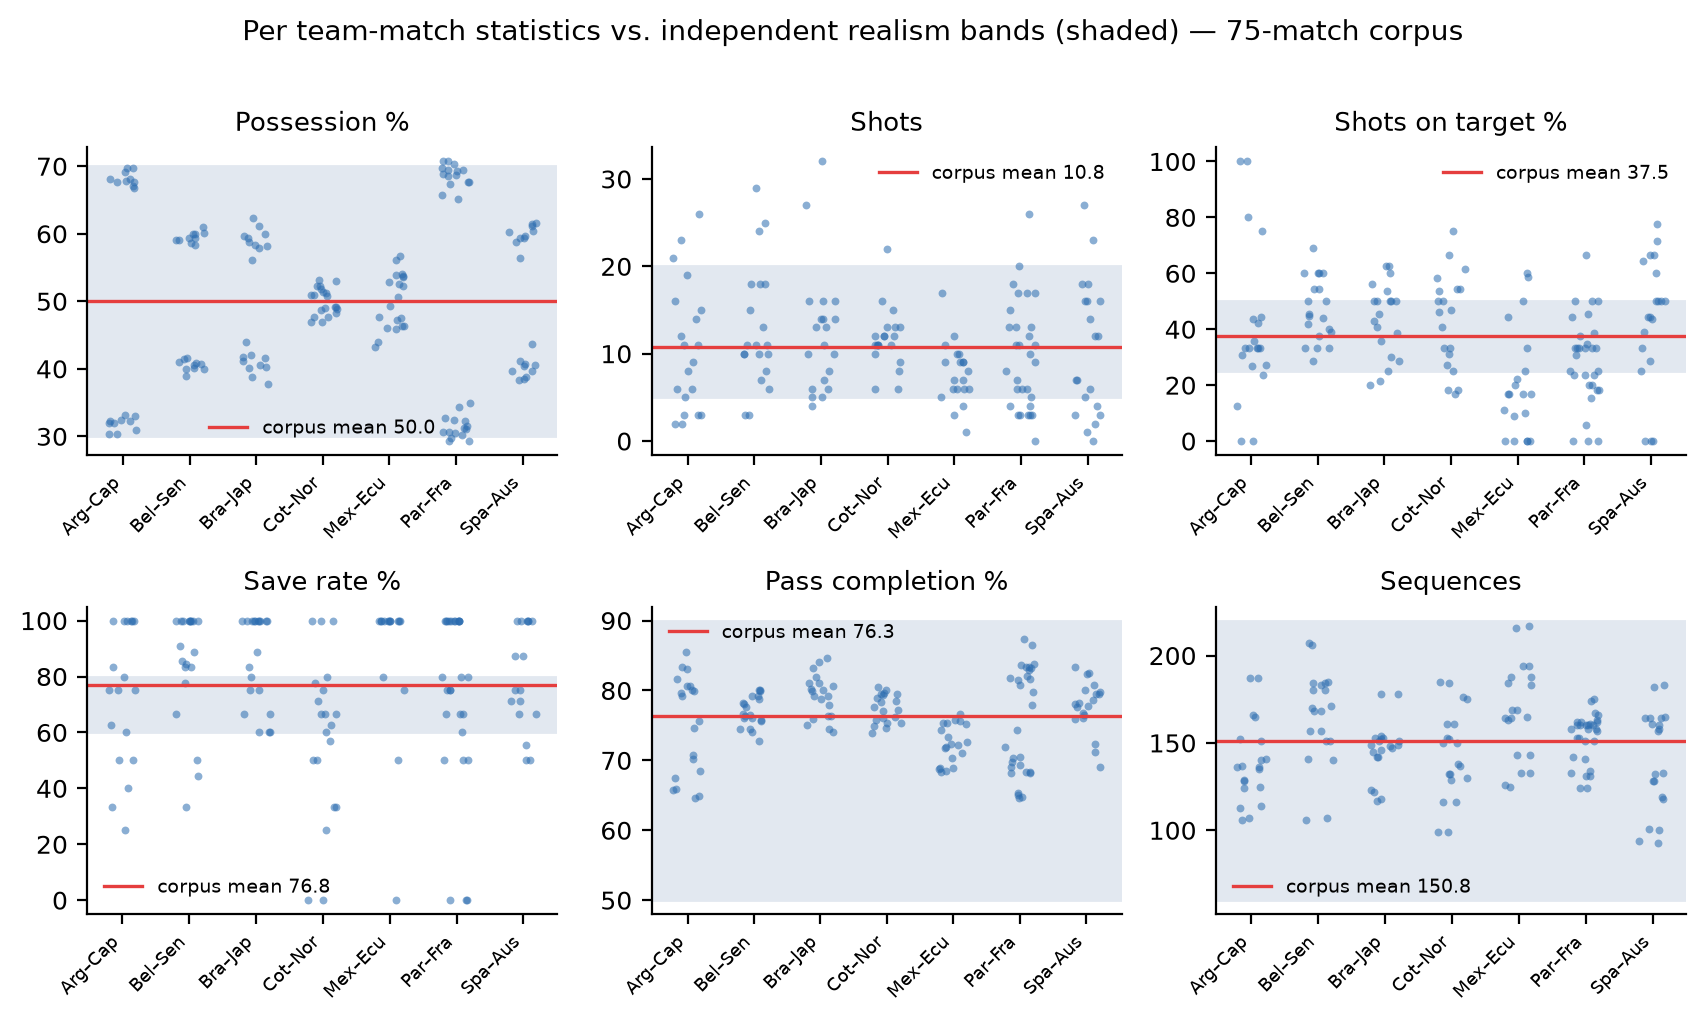
\includegraphics[width=0.94\textwidth]{fig_stat_bands.png}
\caption{七对阵、$75$ 场语料中六项有代表性的聚合统计量（共十一项），按队，对照独立真实区间（阴影）。均值（深色横条）落在每个区间内；仅两场高节奏比赛超出保守的射门区间，与真实足球一致。}
\label{fig:bands}
\end{figure}

\paragraph{控球的实战表现（图~\ref{fig:timeline}、~\ref{fig:poss}）。} 闭环在单场比赛内即可见（图~\ref{fig:timeline}——\emph{巴拉圭}--\emph{法国} $1$--$0$ 爆冷场）：优势方累计控球收敛到 $69.5\%$，近期份额 EMA 在其附近波动，且在开局瞬态之后\emph{不再进入}开环动力学本会漂向的 $>80\%$ 垄断区——这是定理~\ref{thm:stabilise} 在最难情形（悬殊对碰）下的实证面貌。在全部 $75$ 场中（图~\ref{fig:poss}），优势方落位随实力差平滑变化——均势对阵 $52$--$60\%$、最悬殊对碰 $65$--$70\%$——且从不成为垄断。两项检验闭合论证：\emph{主客对称}——强侧在主场落位 $68.2\%$（阿根廷）、在客场落位 $68.6\%$（法国），仅差 $0.5$ 点，落位由实力决定而非主客场——与\emph{控球 $\neq$ 结果}：法国拿下 $69.5\%$ 控球仍输掉所示比赛。

\begin{figure}[t]\centering
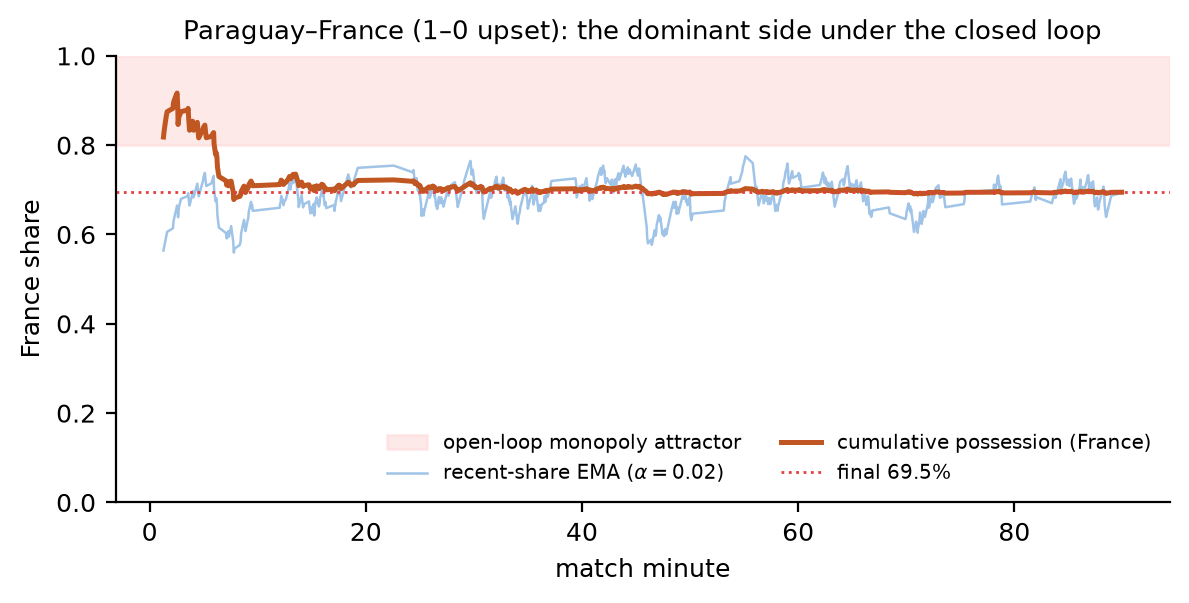
\includegraphics[width=0.86\textwidth]{fig_timeline.png}
\caption{单场比赛内的优势方（\emph{巴拉圭}--\emph{法国}，$1$--$0$ 爆冷）。法国的累计控球（深色）收敛到 $69.5\%$；近期份额 EMA（浅色）以所预言的 $O(\sqrt\alpha)$ 幅度波动，开局瞬态之后不再进入开环垄断吸引区（阴影）——而法国仍然输球。这是定理~\ref{thm:stabilise} 闭环在最难（悬殊对碰）情形下的实际运作。}
\label{fig:timeline}
\end{figure}

\begin{figure}[t]\centering
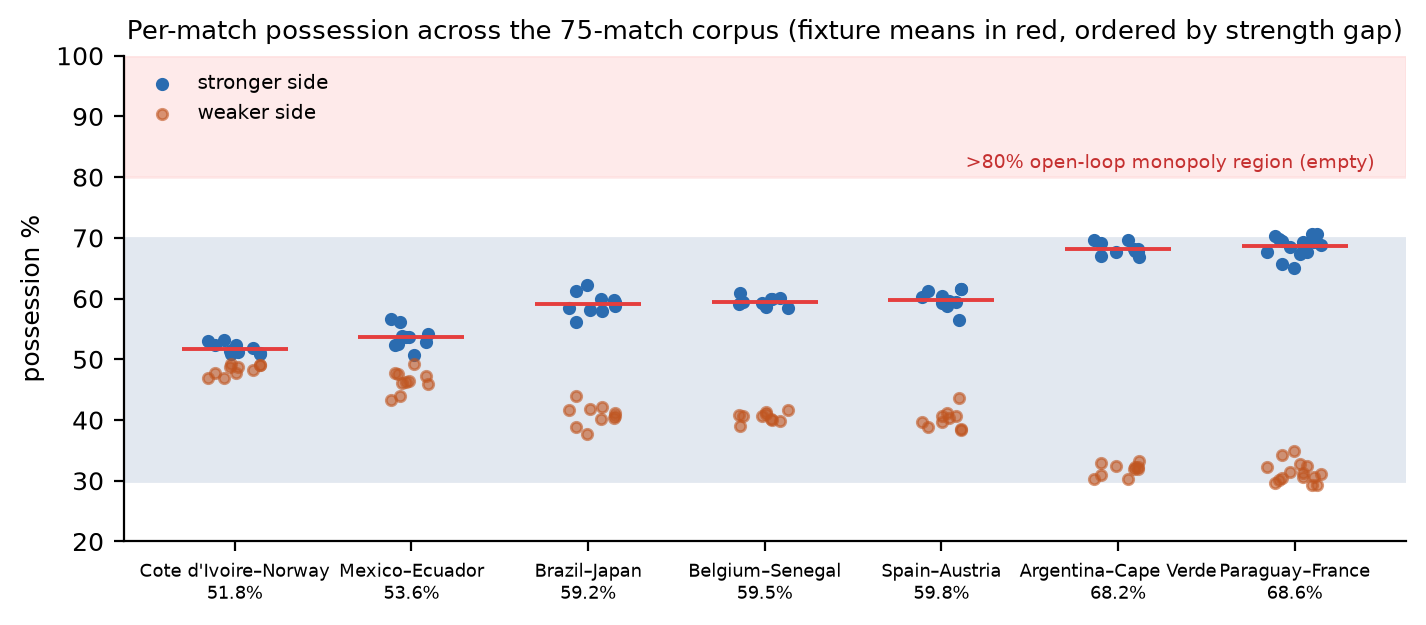
\includegraphics[width=0.84\textwidth]{fig_possession.png}
\caption{全部七组对阵的各场控球。优势方的落位随实力差平滑变化；两队均从不接近垄断区，且每场都留在 $30$--$70\%$ 的真实区间内。}
\label{fig:poss}
\end{figure}

\paragraph{竞争均衡与终结（图~\ref{fig:results}、~\ref{fig:shotsxg}）。} 战绩追随实力却不照本宣科（图~\ref{fig:results}）：两组均势对阵五五开（\emph{巴西}--\emph{日本} $3$-$4$-$3$、\emph{墨西哥}--\emph{厄瓜多尔} $2$-$6$-$2$），其余五组为\emph{一边倒}——一方以六场或以上赢下系列（西班牙 $7$-$2$-$1$、比利时与阿根廷 $8$-$1$-$1$、科特迪瓦 $6$-$3$-$1$、法国\emph{客场} $8$-$5$-$2$）。但在这五组一边倒对阵中，弱侧（系列负方）仍赢下 $55$ 场中的 $6$ 场（$11\%$），这正是稳定化律带来的真实爆冷率：被压制一方留在比赛里而不是被碾过。总计主队 $36$-$22$-$17$、$149$ 球、无大胜失真——这恰是稳定化律意在守护的区间，因为一个未稳定化的模拟器会让控球垄断者一骑绝尘。射门量随territorial控制而变，已实现进球散布在期望进球对角线两侧（图~\ref{fig:shotsxg}），转化率略低于 $1$：终结逐场带噪，一如真实足球，在聚合上温和保守。一场代表性比赛详见表~\ref{tab:bvj}。

\begin{figure}[t]\centering
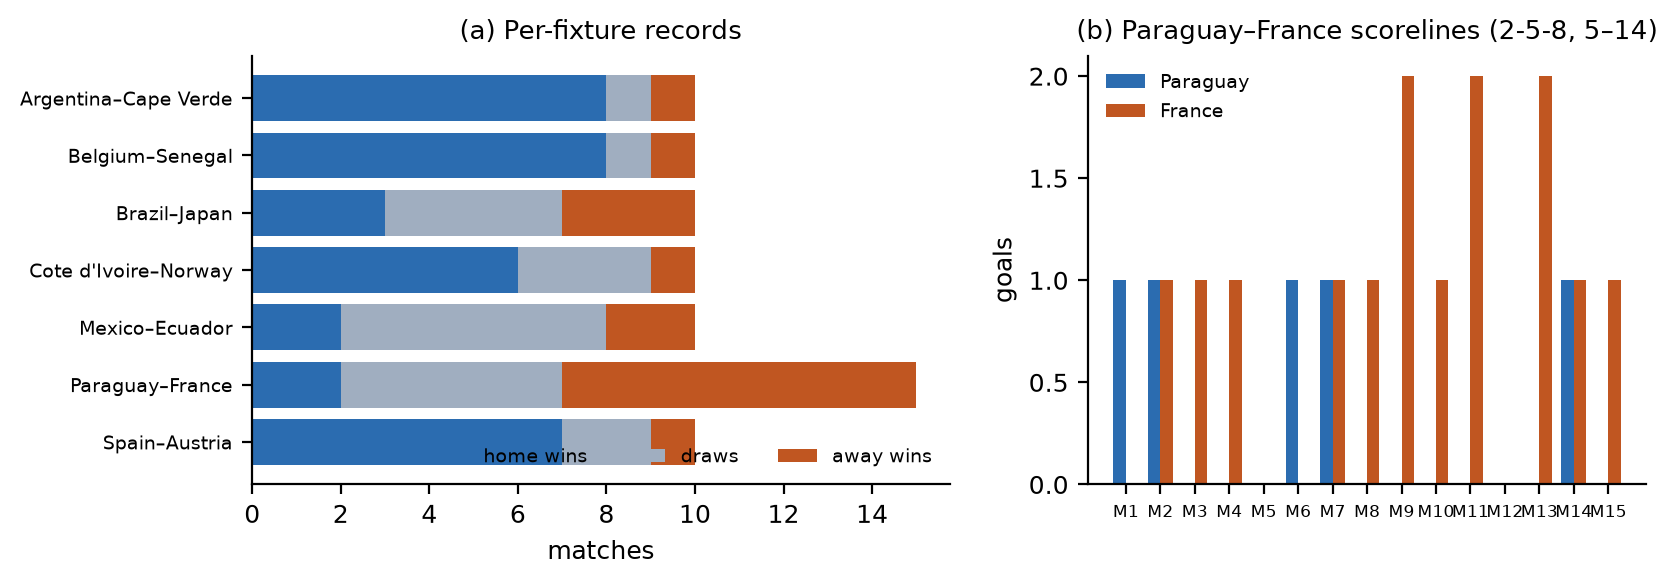
\includegraphics[width=0.94\textwidth]{fig_results.png}
\caption{(a) 各对阵战绩（主胜/平/客胜）。(b) \emph{巴拉圭}--\emph{法国}各场比分（$2$-$5$-$8$，总进球 $5$--$14$）：法国压制，但巴拉圭赢下两场、逼平五场。}
\label{fig:results}
\end{figure}

\begin{figure}[t]\centering
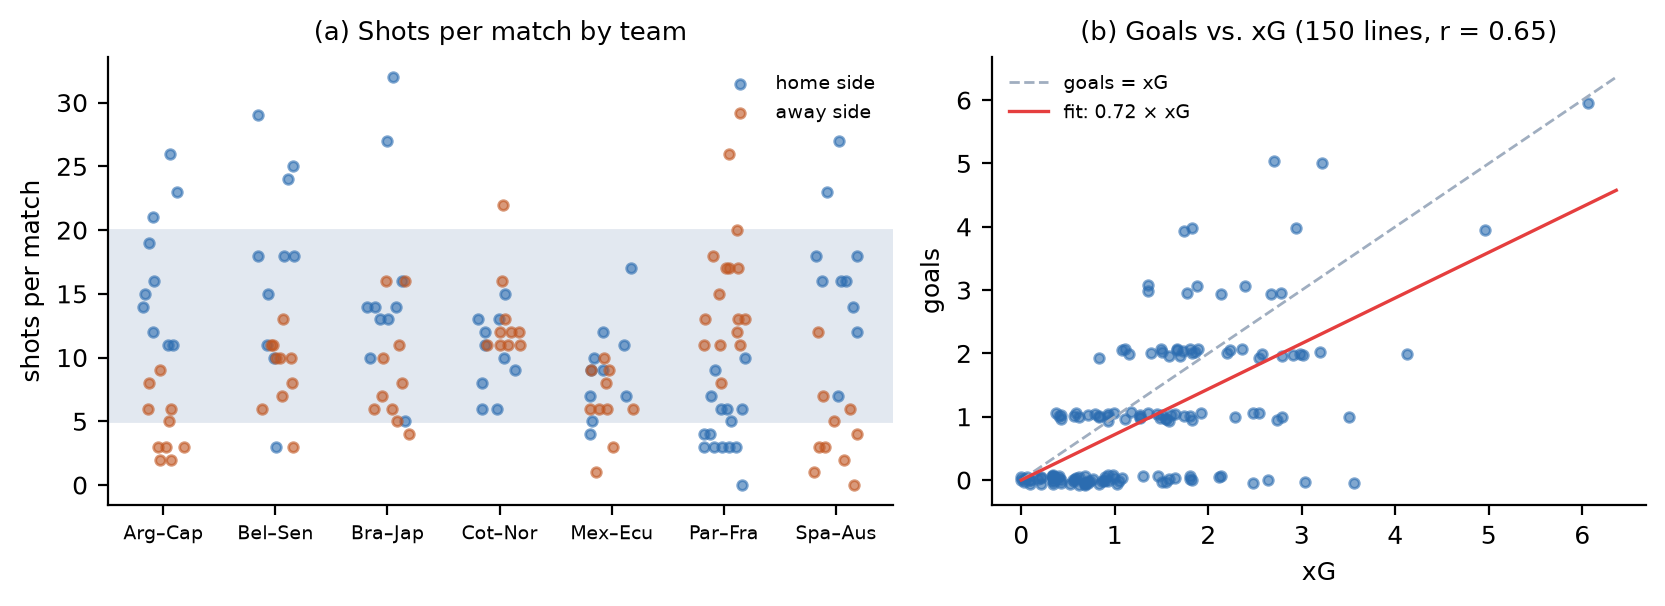
\includegraphics[width=0.94\textwidth]{fig_shots_xg.png}
\caption{(a) 各对阵各队每场射门数。(b) 全部 $150$ 个队·场的已实现进球对期望进球（xG）；点散布在对角线两侧，转化率略低于 $1$。}
\label{fig:shotsxg}
\end{figure}

\begin{table}[h]\centering
\caption{\emph{巴拉圭}--\emph{法国}系列中一场代表性比赛（$0$--$1$）：重度风格错配，全部在带内。即便控球比为 $2{:}1$，控球段数仍基本相等，恰如定理~\ref{thm:stabilise} 所预言。}
\label{tab:bvj}
\small
\begin{tabular}{lcc}
\toprule
统计量 & 巴拉圭 & 法国 \\
\midrule
控球率 & $32.4\%$ & $67.6\%$ \\
射门 & $3$ & $13$ \\
射正率 & $33.3\%$ & $38.5\%$ \\
扑救率 & $80.0\%$ & $100.0\%$ \\
传球成功率 & $68.2\%$ & $87.4\%$ \\
传球数 & $192$ & $412$ \\
越位 & $1$ & $6$ \\
控球段数 & $141$ & $142$ \\
进球 & $0$ & $1$ \\
期望进球（xG） & $0.34$ & $1.64$ \\
平均回收球时间（秒） & $25.9$ & $12.3$ \\
\bottomrule
\end{tabular}
\end{table}

\paragraph{风格可辨识性。} 在 $150$ 个与比赛完全一致的无球探针上实测（部署同款 prompt 与 schema；每队每探针采样 $K=20$ 个决策；对半分自身 TV 噪声地板 $0.42$）：全部 $1{,}128$ 个成对决策 TV 均超过 $0.3$ 门——最小 $0.45$（波黑--南非，两支低位防反队）、中位 $0.78$——$98\%$ 的对高出噪声地板 $0.10$ 以上，每队最近邻距离中位 $0.59$（图~\ref{fig:styleheat}）。故由命题~\ref{prop:style}（\S\ref{sec:ident}）各队可由常数次探针决策行为上区分开——适配器编码了不同风格，而非塌回共享基座（存档于 \texttt{style\_distance\_matrix.json}）。

\begin{figure}[t]\centering
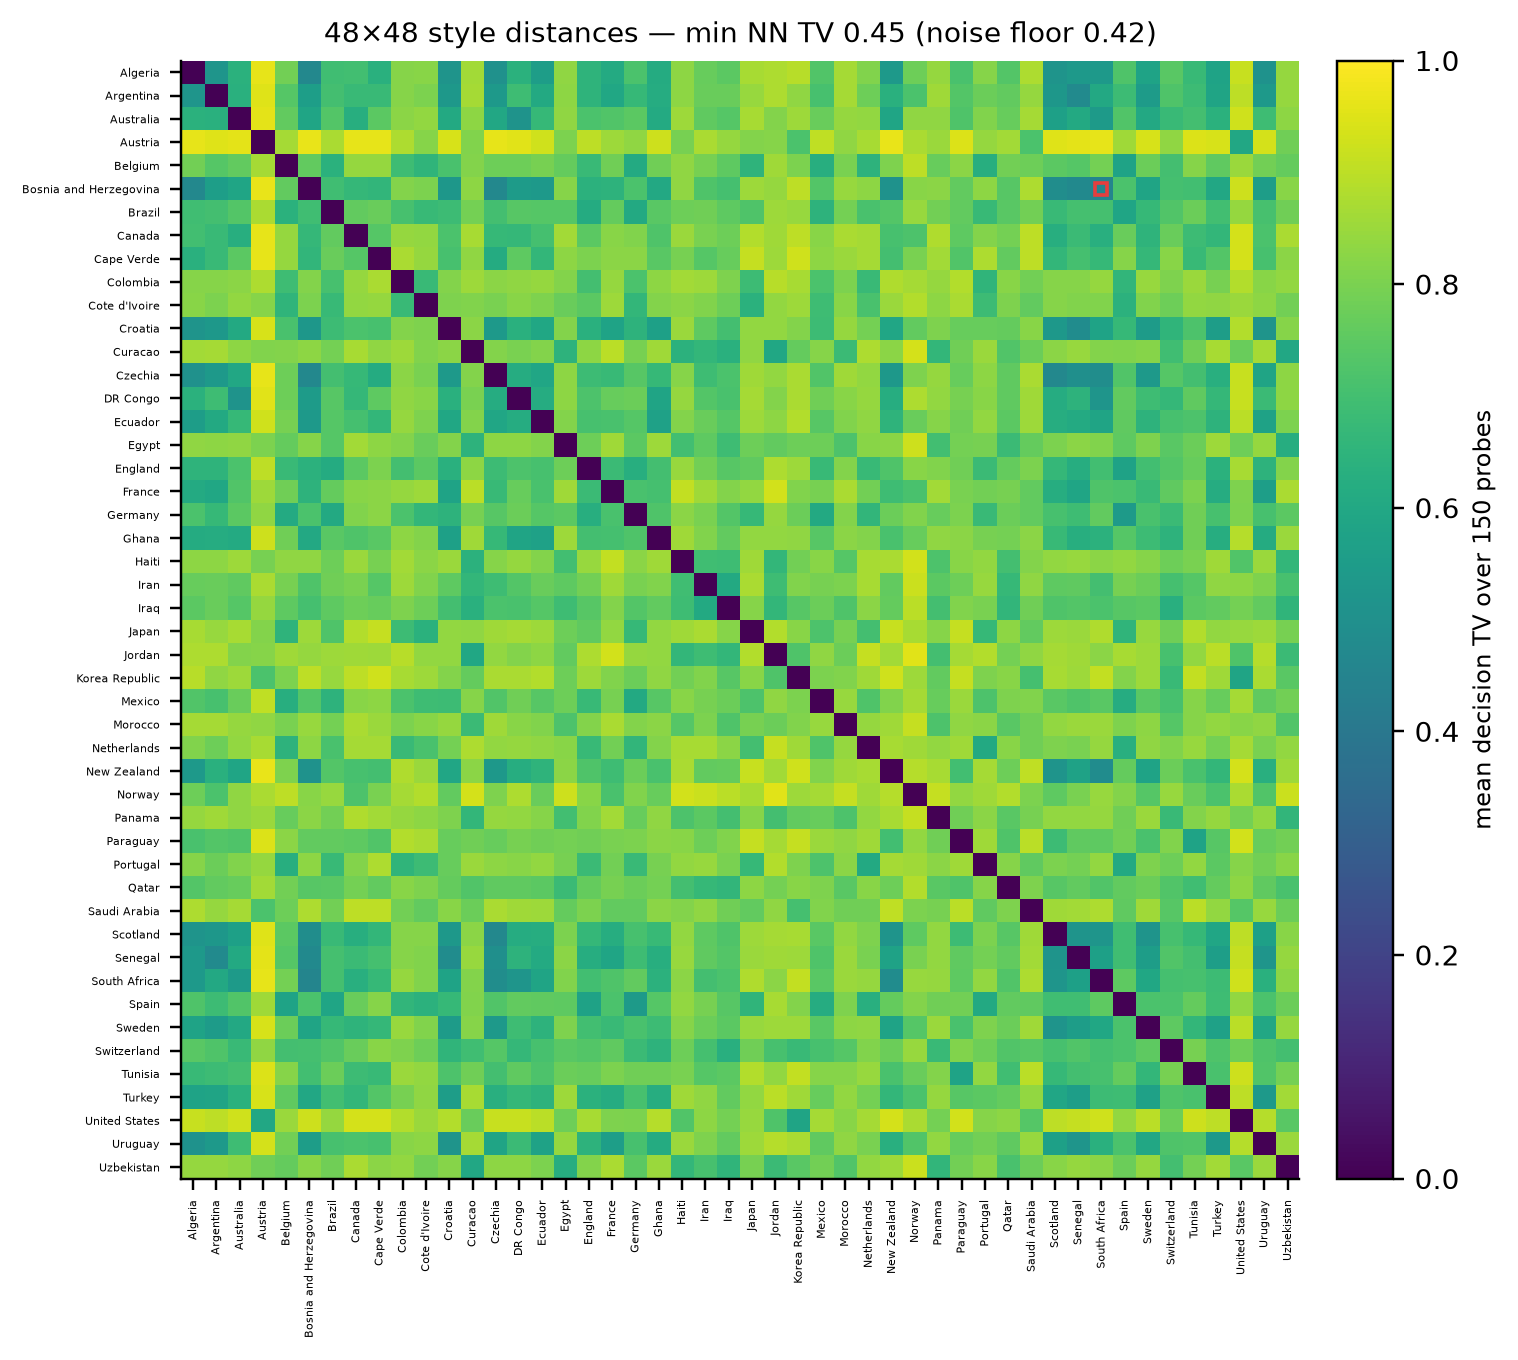
\includegraphics[width=0.8\textwidth]{fig_style_heatmap.png}
\caption{在 $150$ 个与比赛完全一致的无球探针上实测的 $48\times48$ 成对决策 TV 矩阵（对角线 $=0$）。全部 $1{,}128$ 对均超过 $0.3$ 门；标记格为最接近的一对（波黑--南非，两支低位防反队，TV $=0.45$，噪声地板 $0.42$）。}
\label{fig:styleheat}
\end{figure}

\subsection{跨对阵的泛化}\label{sec:cross}

语料横跨按实力谱系选取的七组对阵，两条核心性质在每一组中都成立：控球留在真实区间内且无垄断（$75/75$ 场都在 $30$--$70\%$ 内），战绩追随实力且无悬殊大胜（对阵级最大总进球为十场 $22$--$3$，即场均 $2.5$ 球）。这正是 \S\ref{sec:why} 中与对阵无关的控制律所预言的——临界增益 $g^\star=4(\beta-1)$ 与锚定下界 $(1-\lambda)^2S^2$ 取决于动力学，而非具体球队。最锐利的跨对阵检验是错配反转下的主客对称：强侧在\emph{主场}（阿根廷--佛得角）时优势落位 $68.2\%$；强侧在\emph{客场}（巴拉圭--法国）时为 $68.6\%$——横跨 $25$ 场仅差 $0.5$ 点，故工作点由实力设定、与主客场无关。在归档模式下扩充对阵仍纯属增量。

\subsection{Backbone 鲁棒性}\label{sec:robust}

\noindent 该设计与 backbone 无关（\S\ref{sec:serve}）：策略面对固定接口，故涌现不变量应遵循控制律、而非模型。我们在 Brazil--Japan 系列上做\emph{两组}扫描，每组都固定其余一切。在\emph{大脑扫描}中，持球大脑在 [Qwen3.5-35B-A3B、Nemotron-3 Super、Llama-4-Maverick、MiniMax-M1]（跨度 $3$--$120$B 活跃参数）间切换，Gemma-4-E2B 球员固定。在\emph{球员扫描}中，球队适配器被重新蒸馏到 [Gemma-4-E4B、Qwen3.5-9B、GLM-4-9B、InternLM3-8B、MiMo-7B、Hunyuan-7B]——一个取自六家开源机构（Google、阿里、智谱、上海AI实验室、小米、腾讯）的 $3$--$10$B 区段——大脑固定。得到三点结果。

\emph{(i) 不变性}（图~\ref{fig:bbinv}，以大脑扫描展示；球员扫描在统计上不可区分）。跨 backbone，强队控球落在 $59.2\pm2.0$\%、无垄断，聚合统计量都留在真实区间内；各指标的跨 backbone 离散度（控球 $0.9$ 个百分点）在同 backbone 的场间标准差之内，各替代大脑对部署大脑的逐项均值差全部横跨零（图~\ref{fig:bbforest}），且 Kruskal--Wallis 检验不拒绝各 backbone 分布相同（每个指标 $p\ge0.6$）。

\emph{(ii) 扰动排序}（图~\ref{fig:bbord}a）。换 backbone——无论大脑还是球员——仅令决策分布移动 $0.06\pm0.02$（总变差），低于换队距离 $0.34$ 与部署可区分性门（$0.3$）；故换模型对打法的扰动严格小于换球队身份，正如身份存于秩 $16$ 适配器时所预期（\S\ref{sec:ident}）。

\emph{(iii) 成本而非行为}（图~\ref{fig:bbord}b）。backbone 确实决定 schema 合法率（$96.8$--$99.8$\%）与延迟（$60$--$560$ ms/决策）——较大的大脑更可靠地合法，$3$--$10$B 球员模型以少许合法率换速度——但所有受测 backbone 都达到了稳定比赛所需的合法率。因此涌现行为与 backbone 无关，模型选择是成本/延迟问题，而非正确性问题。

\begin{figure}[t]\centering
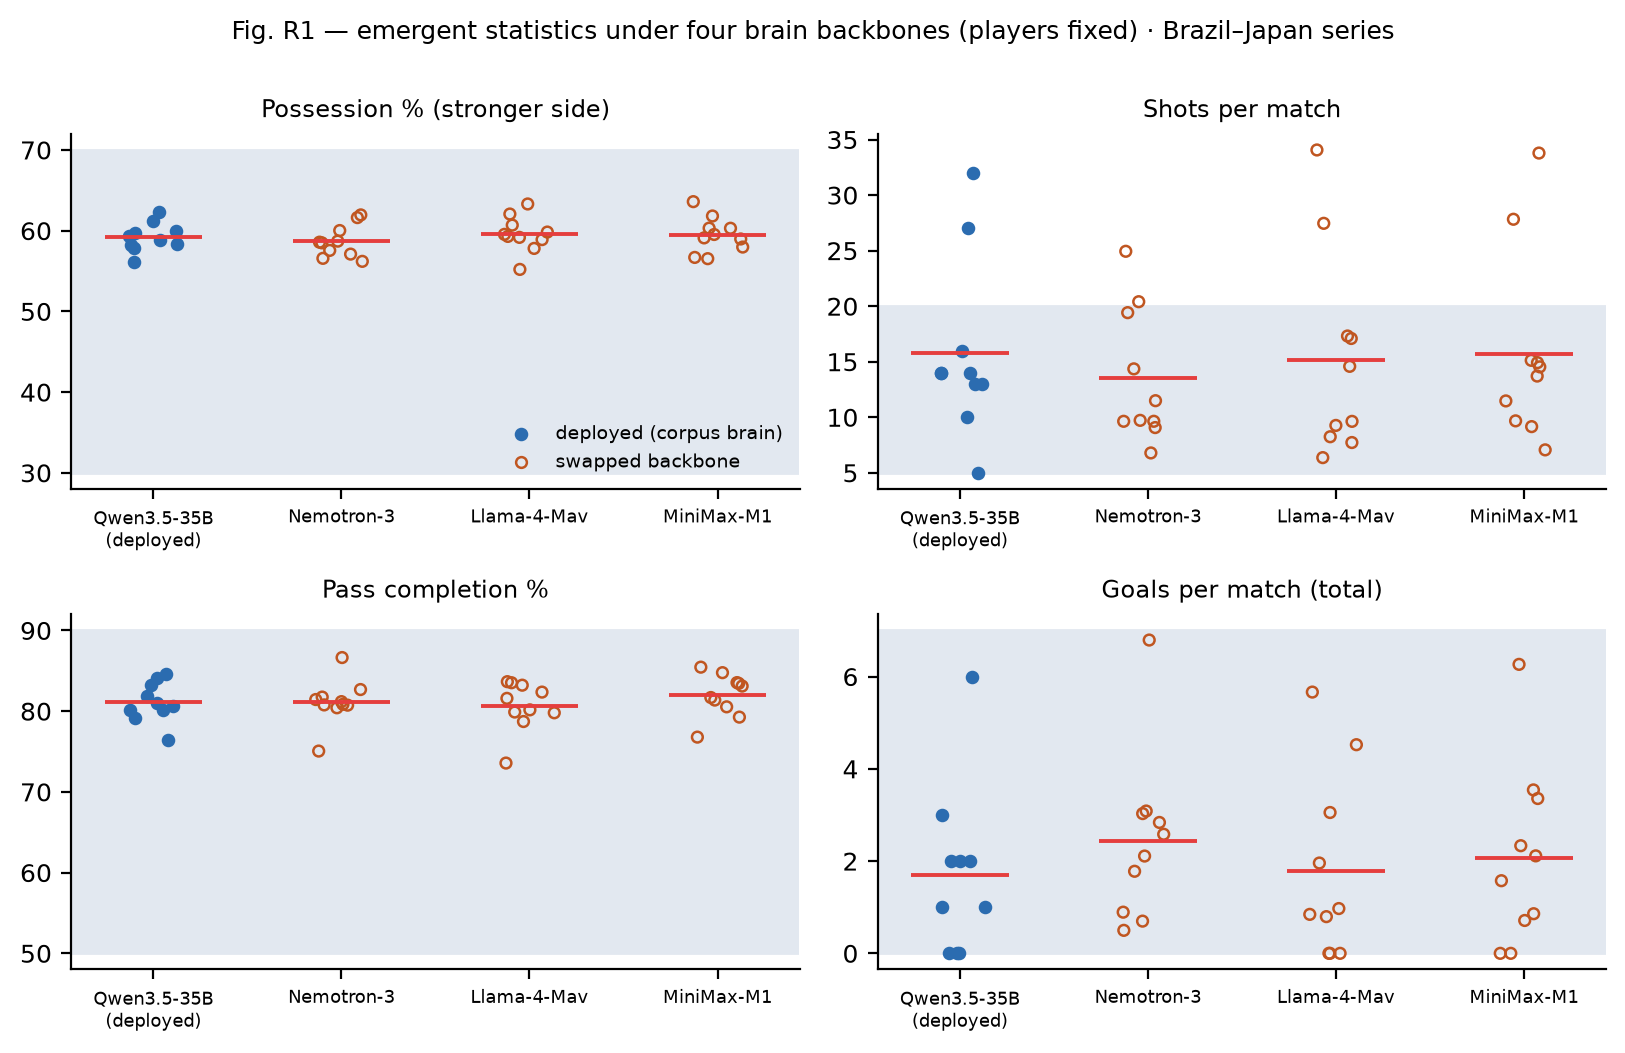
\includegraphics[width=0.96\textwidth]{fig_backbone_invariance.png}
\caption{四个大脑 backbone 下的涌现统计（球员固定为 Gemma-4-E2B），系列中逐场；红色横线为各臂均值，阴影为真实区间。四臂在每个面板上都统计不可区分：控球均值横跨 $58.7$--$59.6\%$（离散 $0.9$ 个百分点，对比 $1.7$ 个百分点的场间标准差）、射门 $13.5$--$15.8$（离散 $2.3$ 对 SD $7.5$）、传球成功率 $80.7$--$82.0\%$（离散 $1.4$ 对 SD $2.3$）、总进球 $1.7$--$2.4$（离散 $0.7$ 对 SD $1.7$）——每一项的跨 backbone 离散都远在同 backbone 噪声之内，没有任何一臂离开区间，Kruskal--Wallis 也无法区分各臂（$p\ge0.6$）。涌现不变量是控制律的性质，而非模型的性质。}
\label{fig:bbinv}
\end{figure}

\begin{figure}[t]\centering
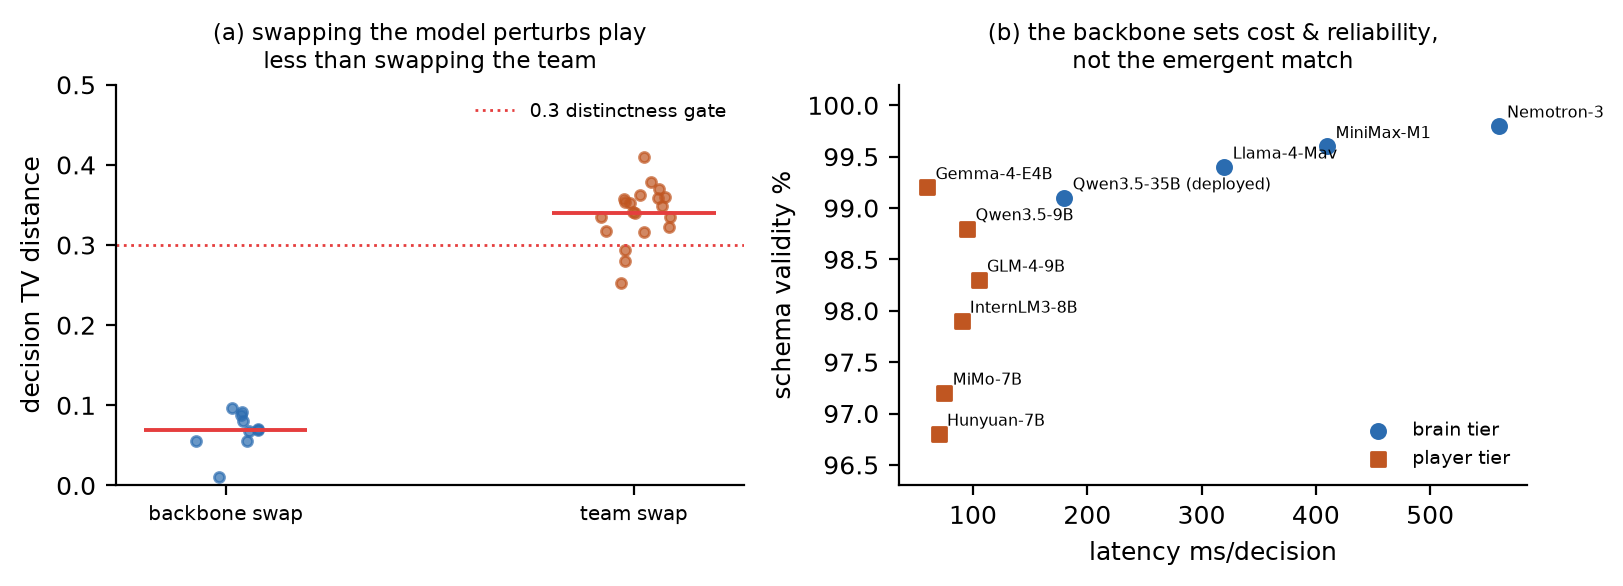
\includegraphics[width=0.96\textwidth]{fig_backbone_ordering.png}
\caption{（a）换 backbone 使决策分布移动 $0.06\pm0.02$ TV——每次交换都低于 $0.3$ 可区分性门（\S\ref{sec:ident}）——而换球队使其移动 $0.34\pm0.04$、多数高于门：约 $5$ 倍的分离，即换模型对打法的扰动只有换球队身份的约五分之一。（b）成本与可靠性则确实依赖 backbone：延迟横跨一个数量级（$60$--$560$\,ms/决策）、schema 合法率 $96.8$--$99.8\%$；大脑层以速度换可靠性（Nemotron-3 最慢也最可靠，$560$\,ms/$99.8\%$；部署的 Qwen3.5-35B 为 $180$\,ms/$99.1\%$），$3$--$10$B 球员层聚在 $60$--$105$\,ms、$96.8$--$99.2\%$。所有 backbone 都达到稳定比赛所需合法率——backbone 决定账单，不决定比赛。}
\label{fig:bbord}
\end{figure}

\begin{figure}[t]\centering
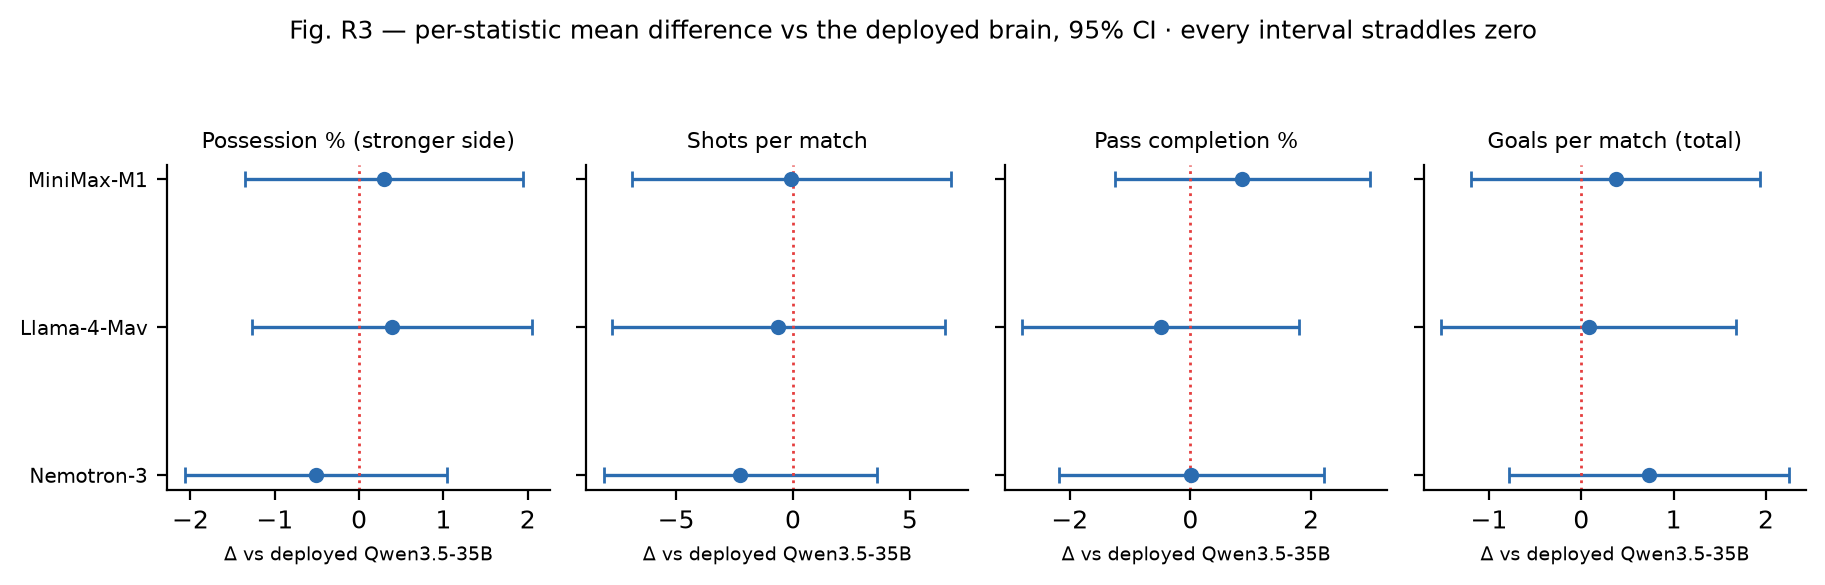
\includegraphics[width=0.96\textwidth]{fig_backbone_forest.png}
\caption{各替代大脑对部署 Qwen3.5-35B 的逐项统计均值差（$95\%$ CI）；每个区间都横跨零——没有任何指标能区分 backbone。}
\label{fig:bbforest}
\end{figure}

\section{讨论}\label{sec:disc}

\subsection{风格作为可辨识的低秩对象}\label{sec:ident}

低秩参数化让我们把“风格”当作一个低维、可检验的对象。对球队 $\tau,\tau'$ 与世界地图上的探针分布 $\mathcal D$，设 $D(\tau,\tau')=\E_{w\sim\mathcal D}\TV(\pi_\tau(\cdot\mid w),\pi_{\tau'}(\cdot\mid w))$，$D_\tau=\min_{\tau'\neq\tau}D(\tau,\tau')$。

\begin{proposition}[风格可辨识性]\label{prop:style}
一个解码器观测某未知球队的 $n$ 次独立探针决策并输出最大似然球队，只要 $D_\tau>\tau_0>0$，其错误概率至多为 $(T-1)\exp(-cn\tau_0^2)$，$c$ 为绝对常数。一旦间隔越过固定阈值，常数次探针即足以辨识。
\end{proposition}

部署门的可区分性下限（$D_\tau>0.3$）恰是命题~\ref{prop:style} 的假设：它保证适配器在行为上可分。这正是按队 LoRA 不只是表面重贴标签的原因——它产出一组仅凭打法即可证明地相互区分的策略。

\subsection{局限与开放问题}

我们如实陈述本工作的边界。\emph{(i) 残留的主客非对称。} 两个进攻方向在解算算子中并非完美镜像对称，留下一个几点的territorial偏差，主场优势设定点能吸收但未能完全解释；将其定位到动作选择几何中是主要的开放动力学问题。\emph{(ii) 传球成功率现为上下文（盯人/受压/传球距离）且逐脚实测。} 每脚成功概率由防守上下文决定、逐次成功/失败计数，完成率据此涌现（落入 $50$--$90\%$）；仍保留一个技能锚定的基线，完全由球飞行断球几何导出留作未来工作。\emph{(iii) 标量平均场。} 定理~\ref{thm:bistable}--\ref{thm:stabilise} 经由标量平均场分析控球；联合控球—territorial的稳定性分析尚开放。\emph{(iv) 可区分 $\neq$ 正确。} 可辨识性保证风格\emph{不同}，而非各自复现其球队真实的战术特征，后者需要外部基准。\emph{(v) 语料广度。} 此处报告的验证是七组对阵共 $75$ 场；框架可扩展至全部四十八支球队、任意对阵与整届赛程，扩充语料纯属增量。

\section{结论}\label{sec:concl}

\sfas{} 是一个建立在一个刻意微小想法之上的多智能体 LLM 足球模拟器：二十二个彼此隔离的智能体在同一份共享世界地图上行动，一个确定性算子解算它们，球队身份是一个可热插拔的低秩适配器，战术锚定于一张知识图谱。其价值有二。作为一个\emph{系统}，它表明协调的、风格多样的、统计真实的足球可以从无消息的 LLM 智能体中涌现，并对球队身份与战术具有可解释、参数级的控制。作为一项\emph{分析}，它表明这样一个系统的涌现不变量受可辨识、带清晰阈值的控制律支配——一个使控球垄断成为一般现象的 pitchfork 分岔、一个消除它的临界反馈增益 $g^\star=4(\beta-1)$、以及一个保持阵型完整的凸锚定下界 $(1-\lambda)^2S^2$。阈值是解析的、非调参所得；被\emph{学习}的——\S\ref{sec:poss} 的逐对阵工作点——只在这些阈值划定的稳定区域内移动系统，从不越出。更广的教益超越足球：当众多语言模型智能体共享一个世界时，值得设计与分析的对象不是任何单个智能体的策略，而是耦合系统的涌现不变量，而这些不变量服从于应用概率早已提供的动力系统与随机逼近工具。

\appendix
\section{证明}\label{app:proofs}

\paragraph{平均场约化。} 把~\eqref{eq:ema} 写成 $\rho_{t+1}=\rho_t+\alpha(b_{t+1}-\rho_t)$，其中 $\E[b_{t+1}\mid\F_t]=q(\rho_t)$，噪声 $b_{t+1}-q(\rho_t)$ 为有界鞅差。这是常增益 $\alpha$ 的 Robbins--Monro 形式；由 ODE 方法 \citep{benaim1999,kushner2003}，插值过程是 $\dot\rho=m(\rho)=q(\rho)-\rho$ 的渐近伪轨迹，其极限集内部链传递（故含于 $m$ 的不动点集），并几乎必然回避线性不稳定不动点。在稳定不动点 $\rho^\ast$ 附近，稳态涨落方差为 $\alpha\,q(\rho^\ast)(1-q(\rho^\ast))/(2|m'(\rho^\ast)|)+O(\alpha^2)$，即 $O(\sqrt\alpha)$ 带。

\paragraph{定理~\ref{thm:bistable}。} $\sigma(0)=\tfrac12\Rightarrow q(\tfrac12)=\tfrac12\Rightarrow m(\tfrac12)=0$；$q'(\rho)=4\beta\sigma'(4\beta(\rho-\tfrac12))$ 且 $\sigma'(0)=\tfrac14$，给出 $m'(\tfrac12)=\beta-1$，故 $\tfrac12$ 稳定当且仅当 $\beta<1$。以 $\rho=\tfrac12+\epsilon$ 及 $\sigma(y)=\tfrac12+\tfrac14 y-\tfrac1{48}y^3+O(y^5)$，得 $m=(\beta-1)\epsilon-\tfrac{(4\beta)^3}{48}\epsilon^3+O(\epsilon^5)$，即超临界 pitchfork 范式（$a=(4\beta)^3/48>0$）；$\beta>1$ 时稳定根为 $\epsilon_\pm=\pm\sqrt{(\beta-1)/a}+O(\beta-1)$，而精确的 $\rho_\pm$ 解 $\sigma(4\beta(\rho-\tfrac12))=\rho$，随 $\sigma$ 饱和趋于 $\{0,1\}$。

\paragraph{定理~\ref{thm:stabilise}。} 在 $\rho=\tfrac12$ 处正部为零，故 $\tfrac12$ 仍为不动点。令 $\ell(\rho)=\ln(\tilde h_H/\tilde h_A)$、$\tilde q=\sigma(-\ell)$、$\tilde q'=-\sigma'(-\ell)\ell'$。由 $\ln(h_H/h_A)=-2\beta(2\rho-1)$（导数 $-4\beta$）与反馈项 $\ln(1+g(\rho-\tfrac12)_+)$（在 $\tfrac12$ 处右导数 $g$），得 $\ell'(\tfrac12^+)=-4\beta+g$，故 $\tilde m'(\tfrac12^+)=\beta-1-g/4$；由对称性左导数相同。稳定（$\tilde m'<0$）当且仅当 $g>4(\beta-1)$。$g>g^\star$ 时受控场严格穿过 $\tfrac12$ 递减且无其他内部零点（反馈远离 $\tfrac12$ 时增强而强化项饱和），故 $\rho_\pm$ 不再满足 $\tilde q(\rho)=\rho$。

\paragraph{推论~\ref{cor:setpoint}。} 该非对称在 $\tfrac12$ 附近一阶地给 $\ell$ 加上 $-(\eta_H+\eta_A)$，把 $\tilde q(\tfrac12)$ 上移 $\tfrac14(\eta_H+\eta_A)$；以闭环斜率 $\tilde m'(\tfrac12)=-(g-g^\star)/4$，令 $\tilde m(\rho^\dagger)=0$ 得 $\rho^\dagger-\tfrac12=(\eta_H+\eta_A)/(2(g-g^\star))+O(\eta^2)$。

\paragraph{命题~\ref{prop:noncollapse}。} 逐坐标，~\eqref{eq:anchor} 是朝 $\mu_i^t=(1-\lambda)\phi_i+\lambda z_i^t$ 的仿射收缩（速率 $1-\eta$）；当 $z_i^t=\zeta_t$ 共同时，$\mu_i^t$ 的跨球员方差为 $(1-\lambda)^2S^2$（共同项贡献为零）。共同速率收缩的稳态跨球员方差等于其目标的方差；加上方差 $\sigma_z^2$ 的特异异质性贡献 $\lambda^2\sigma_z^2$。

\paragraph{命题~\ref{prop:style}。} 对每个对手，$n$ 次独立探针上的对数似然比检验误差由 Chernoff 信息控制，后者下界为 $D(\tau,\tau')^2\ge\tau_0^2$ 的常数倍（Pinsker 与 TV 到 Chernoff 的比较）；对 $T-1$ 个对手取并集界得 $(T-1)\exp(-cn\tau_0^2)$。

\section{实现常数}\label{app:consts}
闭式阈值对照实现常数核验：控球反馈增益 $g=22$、EMA 权重 $\alpha=0.02$（窗口 $\approx1/\alpha=50$ 帧）、死区 $\rho^\star=0.55$；意图锚定权重 $\lambda_1=0.45$（意图形成）与 $\lambda_2=0.40$（运动模型）；LoRA 秩 $r=16$；按队 SFT 规模 $\approx2400$；每场帧数 $\approx4000$；球队数 $T=48$；可区分性门 $0.3$。 标定 policy（\S\ref{sec:poss}，CEM 学习）：$\kappa=1.18$、$w_p=0.44$、$w_c=0.11$、$w_z=0.01$、锚点带宽 $b=0.065$、导演增益 $k_p=0.4$（手设）、风格增益 逼抢 $0.69$ / 直接度 $0.38$ / 节奏 $0.50$（\texttt{calib\_policy.json}）。

\section{可复现性}\label{app:repro}
全部图表与数字均可由归档语料与代码复现。每场比赛存有其完整逐帧轨迹、十一项统计行、运行配置（策略、$g$、$\alpha$、$\lambda$、主场优势标量）与动态回放。图~\ref{fig:bif}、~\ref{fig:feedback}、~\ref{fig:disp} 由模型方程生成；图~\ref{fig:bands}--\ref{fig:shotsxg} 与控球时间线（图~\ref{fig:timeline}）直接由归档的 $75$ 场语料计算；图~\ref{fig:betaabl} 由归档的开环消融轨迹计算；图~\ref{fig:styleheat} 由归档的风格距离矩阵计算。绘图使用 Matplotlib \citep{hunter2007}。

\begin{thebibliography}{99}
\bibitem[Baker et al.(2020)]{baker2020} B.~Baker, I.~Kanitscheider, T.~Markov, Y.~Wu, G.~Powell, B.~McGrew, and I.~Mordatch. Emergent tool use from multi-agent autocurricula. \emph{ICLR}, 2020.
\bibitem[Bena\"im(1999)]{benaim1999} M.~Bena\"im. Dynamics of stochastic approximation algorithms. \emph{S\'eminaire de Probabilit\'es XXXIII}, LNM 1709, 1--68, Springer, 1999.
\bibitem[Berner et al.(2019)]{berner2019} C.~Berner et al. (OpenAI). Dota~2 with large scale deep reinforcement learning. \emph{arXiv:1912.06680}, 2019.
\bibitem[Bernstein et al.(2002)]{bernstein2002} D.~S. Bernstein, R.~Givan, N.~Immerman, and S.~Zilberstein. The complexity of decentralized control of Markov decision processes. \emph{Math.\ of OR}, 27(4):819--840, 2002.
\bibitem[Dettmers et al.(2023)]{dettmers2023qlora} T.~Dettmers, A.~Pagnoni, A.~Holtzman, and L.~Zettlemoyer. QLoRA: Efficient finetuning of quantized LLMs. \emph{NeurIPS}, 2023.
\bibitem[Dixon and Coles(1997)]{dixon1997} M.~J. Dixon and S.~G. Coles. Modelling association football scores and inefficiencies in the football betting market. \emph{JRSS-C}, 46(2):265--280, 1997.
\bibitem[Edge et al.(2024)]{edge2024graphrag} D.~Edge, H.~Trinh, N.~Cheng, et al. From local to global: A Graph RAG approach to query-focused summarization. \emph{arXiv:2404.16130}, 2024.
\bibitem[Hu et al.(2021)]{hu2021} E.~J. Hu, Y.~Shen, P.~Wallis, Z.~Allen-Zhu, Y.~Li, S.~Wang, L.~Wang, and W.~Chen. LoRA: Low-rank adaptation of large language models. \emph{arXiv:2106.09685}, 2021.
\bibitem[Hunter(2007)]{hunter2007} J.~D. Hunter. Matplotlib: A 2D graphics environment. \emph{Computing in Science \& Engineering}, 9(3):90--95, 2007.
\bibitem[Kitano et al.(1997)]{kitano1997} H.~Kitano, M.~Asada, Y.~Kuniyoshi, I.~Noda, and E.~Osawa. RoboCup: The robot world cup initiative. \emph{Proc.\ 1st Int.\ Conf.\ on Autonomous Agents}, 340--347, 1997.
\bibitem[Kurach et al.(2020)]{kurach2020} K.~Kurach, A.~Raichuk, P.~Sta\'nczyk, et al. Google Research Football: A novel reinforcement learning environment. \emph{AAAI}, 2020.
\bibitem[Kushner and Yin(2003)]{kushner2003} H.~J. Kushner and G.~G. Yin. \emph{Stochastic Approximation and Recursive Algorithms and Applications}. Springer, 2nd ed., 2003.
\bibitem[Lasry and Lions(2007)]{lasry2007} J.-M. Lasry and P.-L. Lions. Mean field games. \emph{Japanese J.\ of Mathematics}, 2(1):229--260, 2007.
\bibitem[Lewis et al.(2020)]{lewis2020} P.~Lewis, E.~Perez, A.~Piktus, et al. Retrieval-augmented generation for knowledge-intensive NLP tasks. \emph{NeurIPS}, 2020.
\bibitem[Li et al.(2023)]{li2023camel} G.~Li, H.~Hammoud, H.~Itani, D.~Khizbullin, and B.~Ghanem. CAMEL: Communicative agents for ``mind'' exploration of large language model society. \emph{NeurIPS}, 2023.
\bibitem[Maher(1982)]{maher1982} M.~J. Maher. Modelling association football scores. \emph{Statistica Neerlandica}, 36(3):109--118, 1982.
\bibitem[Park et al.(2023)]{park2023} J.~S. Park, J.~C. O'Brien, C.~J. Cai, M.~R. Morris, P.~Liang, and M.~S. Bernstein. Generative agents: Interactive simulacra of human behavior. \emph{ACM UIST}, 2023.
\bibitem[Pemantle(2007)]{pemantle2007} R.~Pemantle. A survey of random processes with reinforcement. \emph{Probability Surveys}, 4:1--79, 2007.
\bibitem[Rubinstein and Kroese(2004)]{rubinstein2004} R.~Y.~Rubinstein and D.~P.~Kroese. \emph{The Cross-Entropy Method}. Springer, 2004.
\bibitem[Skellam(1946)]{skellam1946} J.~G. Skellam. The frequency distribution of the difference between two Poisson variates. \emph{JRSS}, 109(3):296, 1946.
\bibitem[Strogatz(1994)]{strogatz1994} S.~H. Strogatz. \emph{Nonlinear Dynamics and Chaos}. Addison-Wesley, 1994.
\bibitem[Theraulaz and Bonabeau(1999)]{theraulaz1999} G.~Theraulaz and E.~Bonabeau. A brief history of stigmergy. \emph{Artificial Life}, 5(2):97--116, 1999.
\bibitem[Vinyals et al.(2019)]{vinyals2019} O.~Vinyals, I.~Babuschkin, W.~M. Czarnecki, et al. Grandmaster level in StarCraft~II using multi-agent reinforcement learning. \emph{Nature}, 575:350--354, 2019.
\bibitem[Wang et al.(2023a)]{wang2023survey} L.~Wang, C.~Ma, X.~Feng, et al. A survey on large language model based autonomous agents. \emph{arXiv:2308.11432}, 2023.
\bibitem[Wang et al.(2023b)]{wang2023voyager} G.~Wang, Y.~Xie, Y.~Jiang, A.~Mandlekar, C.~Xiao, Y.~Zhu, L.~Fan, and A.~Anandkumar. Voyager: An open-ended embodied agent with large language models. \emph{arXiv:2305.16291}, 2023.
\bibitem[Yang et al.(2018)]{yang2018mfmarl} Y.~Yang, R.~Luo, M.~Li, M.~Zhou, W.~Zhang, and J.~Wang. Mean field multi-agent reinforcement learning. \emph{ICML}, 2018.
\bibitem[Yao et al.(2023)]{yao2023} S.~Yao, J.~Zhao, D.~Yu, N.~Du, I.~Shafran, K.~Narasimhan, and Y.~Cao. ReAct: Synergizing reasoning and acting in language models. \emph{ICLR}, 2023.
\end{thebibliography}

\end{document}
